\chapter{Fundamentação Teórica}\label{cap:fundTeo}

\section{Inteligência Artificial}

\subsection{Um pouco sobre a Historia}
%-
O termo inteligência artificial foi expressa pela primeira vez por Alan Turing em 1950, ano no qual ele lançou um artigo falando sobre o seu “jogo da imitação”, hoje conhecido como “Teste de Turing”, já na época ele reconhece vários desafios a serem vencidos, inclusive com uma frase emblemática “as maquinas podem pensar” [19].
 \begin{quotation}
    \footnotesize Acredito que, em cerca de 50 anos, será possível programar computadores, com uma capacidade de memória de cerca de \(10^9\) \cite{alanT} tradução nossa.
 \end{quotation}
O que é inteligência artificial? Este assunto tem intrigado várias áreas de estudo como a biologia, psicologia, filosofia, talvez uma maneira simples de definir é dizer que, a  inteligência artificial ou “IA” é um campo de pesquisa da tecnologia que relaciona conceitos da fisiologia humana, alguns mais simples como os próprios sentidos,  um exemplo é a visão e outros conceitos mais focados na capacidade do ser humano em conseguir raciocinar para tomar certas atitudes na solução de problemas complexos, por exemplo no caso da visão como conseguimos distinguir um objeto de outros, um indiviso de outro, etc. A inteligência artificial nada mais é do que a tentativa de imitar o comportamento humano em máquinas programas [20].
O conceito de aprendizado de máquina é muito importante em IA pois ele agrega os conceitos de treinamento: aprender a interpretar entradas que vem em conjuntos finitos ou infinitos, classificá-los e assim gerar uma resposta ou como e mais conhecido uma saída de dados. Aprendizado por hábito: capacidade de um computador realizar alguma função logica (A) e armazená-la como dado para posteriormente utilizá-la como referência para poder reagir a uma função semelhante a função (A), isso e conhecido em inteligência artificial como uma rede neural.  [20].

%-
\subsection{Machine Learnig}
%-
Machine Learning ou aprendizado de máquina é uma subárea da inteligência artificial, ela surgiu por volta dos anos 1980 junto com a impulsão de novos computadores quando eles começaram a evoluir em termos de hardware e processamento [21]. Em aprendizado de máquina, computadores são programados para aprender e evoluir com processos anteriores, para isso eles utilizam inferência que se denomina indução, eles obtêm conclusões genéricas se baseando em exemplos armazenados nos processos anteriores. Assim o algoritmo aprende a induzir uma função que será um problema a ser resolvido, a partir de experiências anteriores que são chamados de dados [21]. Alguns exemplos bem-sucedidos:
\begin{itemize}
    \item Reconhecimento de palavras;
    \item Predição de taxa de cura de pacientes;
    \item Detecção de fraudes em cartões de crédito;
    \item Veículos autônomos;
    \item Jogos de xadrez autônomo;
    \item Diagnóstico de câncer por análise de dados por expressão genica;
\end{itemize}
%-
\subsection{Deep Learnig}
%-
Deep Learning ou aprendizado aprofundado e uma subárea do aprendizado de máquina é um conceito que utiliza redes neurais artificias para que a máquina consiga não só resolver problemas, mas também aprender novas maneiras de resolvê-los [22].  E um conceito que estuda uma maneira de imitar o funcionamento dos neurônios humanos e contextualizá-los em modelos matemáticos, utilizando modelagem cognitiva a partir da mente humana. Esse estudo deu origem ao conceito de redes neurais artificiais e quando falamos de Deep Learning estamos nos referindo diretamente a redes neurais [22].
A figura \ref{fig:exRedeNeural} mostra os vários modelos de redes neurais desde o primeiro modelo que seria um perceptron, que é basicamente um ramo de uma rede foi o primeiro modelo, até conceitos mais profundos de redes neurais [22].

\begin{figure}[H]
  \centering
  \caption{Exemplo de Redes Neurais}
  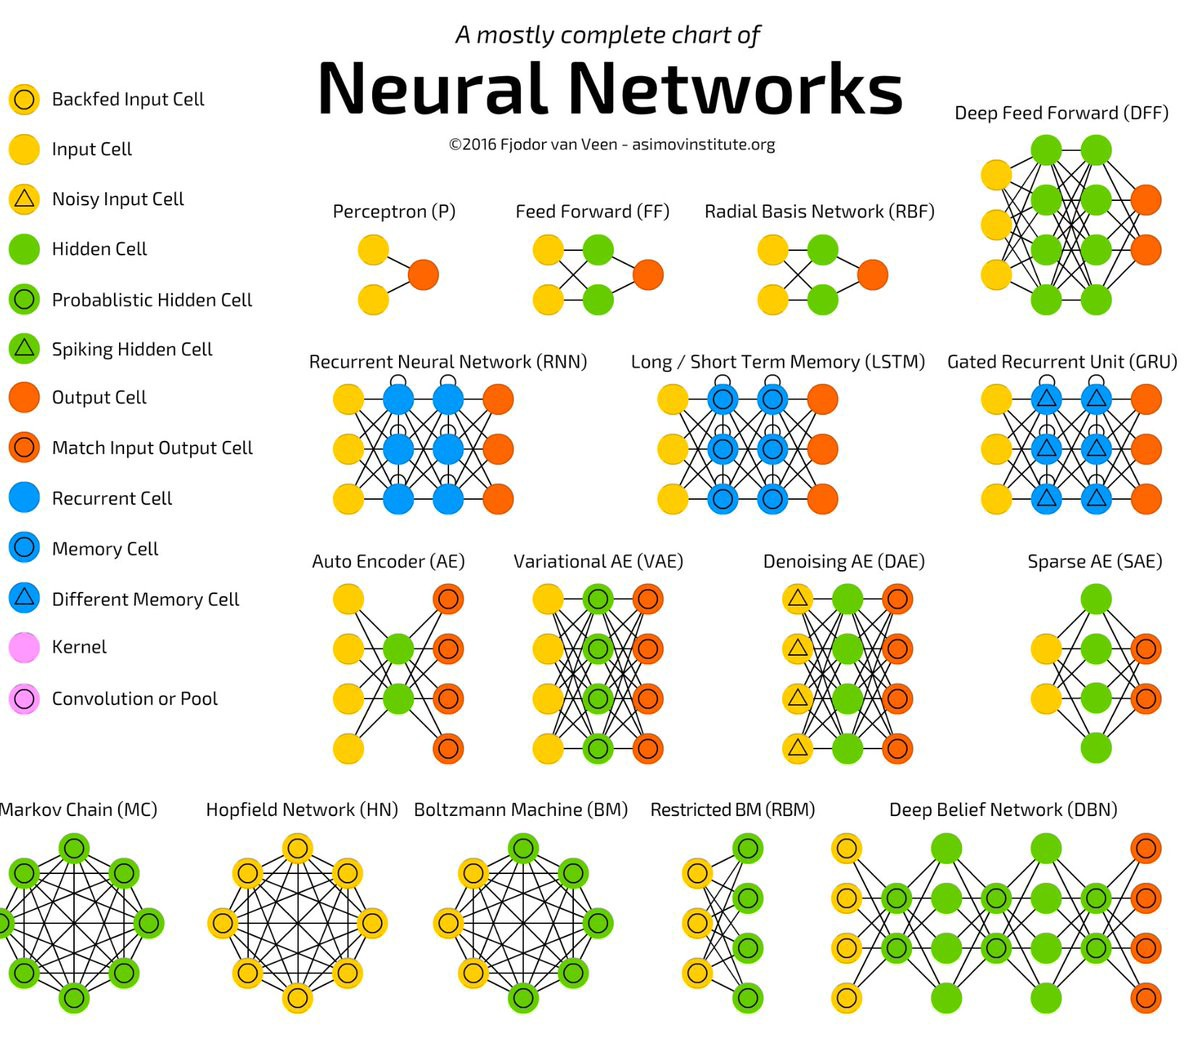
\includegraphics[scale=.2]{figs/neuralNetwork.jpg}
  \legend{Fonte: GitBook, \cite{exRedeNeural}.}
  \label{fig:exRedeNeural}
\end{figure}

A figura \ref{fig:iamldl} mostra um exemplo da diferença entre Inteligência Artificial, Machine Learning e Deep Learning, e quando aproximadamente elas começaram a ser abordadas e implementadas.

\begin{figure}[H]
  \centering
  \caption{Diferença entre IA, ML e DL}
  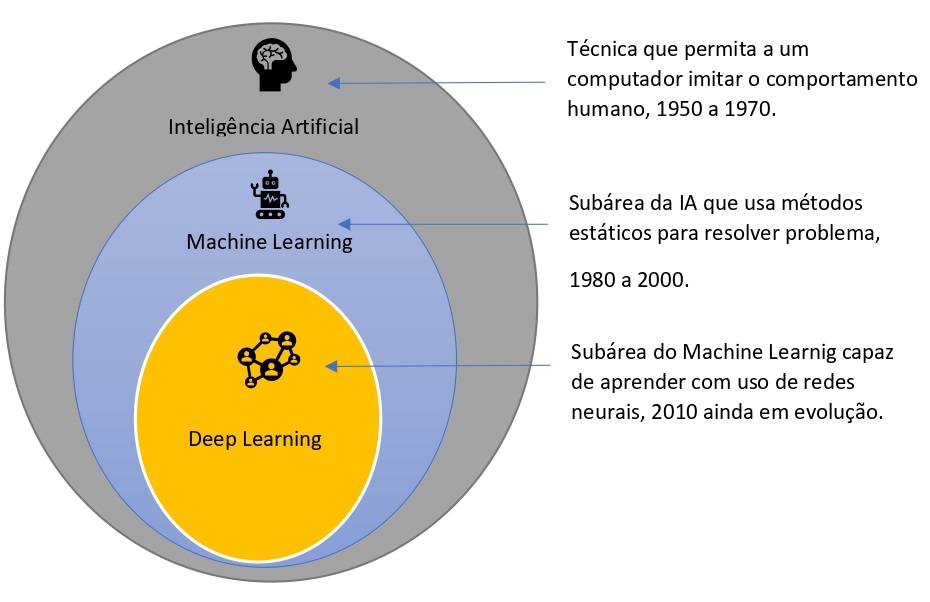
\includegraphics[scale=.7]{figs/IA-ML-DL.jpg}
  \legend{Fonte: o autor.}
  \label{fig:iamldl}
\end{figure}

Uma rede neural nada mais é do que uma maneira de imitar o que ocorre no cérebro humana quando realizamos tarefas e assim ativamos neurônios que por sua vez ativam outros, e assim realizando uma reação em cadeia que gera o que chamamos de pensamento. A figura \ref{fig:neural} é um simples exemplo de uma rede neural em máquinas aonde existem entradas, que ativam neurônios, que por sua vez se ligam com todos os outros neurônios e assim sucessivamente até chegarem em apenas uma saída [20].

\begin{figure}[htpb]
  \centering
  \caption{Rede Neural}
  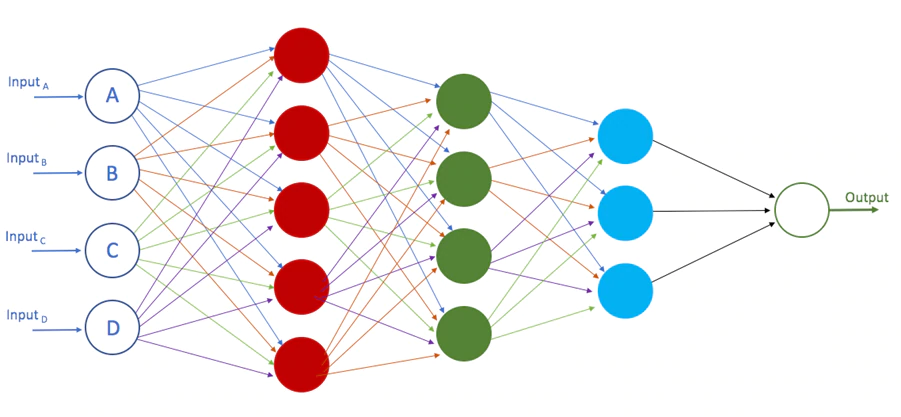
\includegraphics[scale=.5]{figs/neural.png}
  \legend{Fonte: Oracle. \cite{neural}.}
  \label{fig:neural}
\end{figure}
%-
\subsection{Visão Computacional}
%-
Visão computacional é um campo da inteligência artificial que treina computadores para interpretar e entender o mundo visual. Através do uso de imagens digitais de câmeras e vídeos, junto a modelos de Deep Learning, as máquinas podem identificar e classificar objetos corretamente — e, então, reagir ao que elas “veem.” [10].
Os estudos com visão computacional beiram a época do início da internet, sim isso e verdade já naquela época se estudava este campo, porem tudo era mais difícil, devido à falta de tecnologias para suportar o processamento de grande volume de dados, faltava o volume de dados hoje conhecido como (Big Data) e algoritmos de processamento paralelo [9]. Nessa década vários fatores impulsionam o uso e estudo de visão computacional, tecnologias moveis saturam o mundo com vídeos e fotos o (Big data), o poder computacional cresceu abruptamente e tornou-se mais barato, e novos algoritmos com redes neurais convulsionais aproveitam melhor a capacidade do hardware e do software [10].
 Existem muitos tipos de visão computacional. Hoje no mercado é comum a utilização de algumas tecnologias distintas, tais como:

\begin{itemize}
    \item Segmentação de imagem: Examina uma fração de uma imagem.
    \item Detecção de objetos: Detecta um os mais objetos dentro de um campo de imagem.
    \item Reconhecimento facial: Detecção avançada de objetos que pode distinguir indivíduos.
    \item Deslocamento dinâmico de objetos: Detecta a reorganização de pixels dentro de um campo de imagem (biblioteca NumPy).
\end{itemize}
%-
\subsection{Redes Neurais Profundas (Deep Learning)}
%-
Aprendizagem Profunda ou Deep Learning, é uma subárea da Aprendizagem de Máquina, que emprega algoritmos para processar dados e imitar o processamento feito pelo cérebro humano [9].
Deep Learning nada mais é do que uma evolução das redes neurais, através da utilização de algoritmos de aprendizagem e camadas de aprendizagem cria-se modelos capazes de reconhecer padrões.
Existem várias arquiteturas de redes neurais, uma é a rede neural convolucional profunda demonstrada na figura \ref{fig:neuralConv}, este tipo trabalha muito bem com entrada de dados multidimensional ou espacial que é o caso do tratamento de imagens. 

\begin{figure}[H]
  \centering
  \caption{Rede Neural Convolucional}
  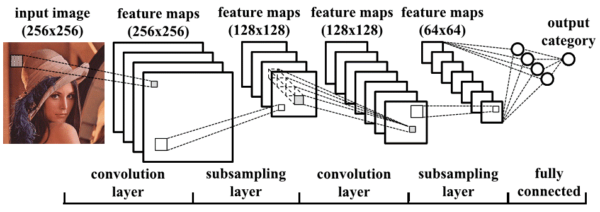
\includegraphics[scale=.6]{figs/neuralConv.png}
  \legend{Fonte: Lambda3, \cite{neuralConv}}
  \label{fig:neuralConv}
\end{figure}

Em visão computacional as entradas são matrizes tridimensionais contendo altura e largura e profundidade, o que determina o padrão ou canal de cor do pixel, a figura \ref{fig:pixel} demonstra esse padrão.

\begin{figure}[htpb]
  \centering
  \caption{Pixel em Visão Computacional}
  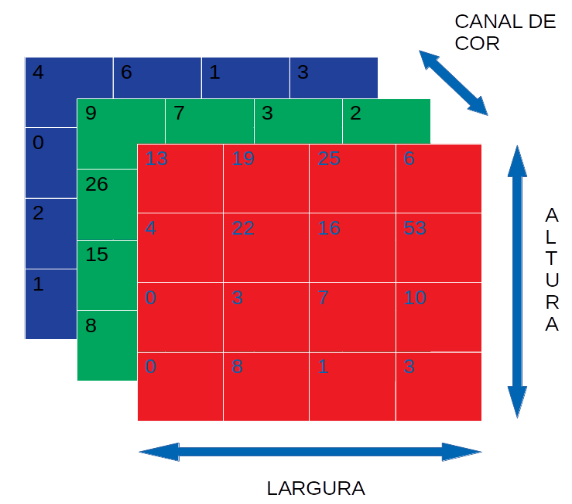
\includegraphics[scale=.9]{figs/pixel.png}
  \legend{Fonte: o autor.}
  \label{fig:pixel}
\end{figure}

A primeira coisa que precisamos para treinar um algoritmo de Deep Learning ée de uma grande quantidade de imagens (Big data), e através de uma abordagem supervisionada com imagens devidamente marcadas como sendo o rosto que buscamos assim realizamos o treinamento. Então teremos um modelo que recebera imagens não marcadas e ele deverá ser capaz de classificá-las.
%-
\section{Tecnologias Open Source para Tratamento de Imagens}
%\addcontentsline{toc}{section}{Trabalhos Relacionados a Isto}

\subsection{OpenCV}
%-
O OpenCV é uma biblioteca de código aberto licenciada por BSD que inclui várias centenas de algoritmos de visão computacional.
Foi iniciada pela Intel em 1999, é uma biblioteca multiplataforma concentra seu foco no processamento de imagens em tempo real e inclui implementações sem patentes e possui todos os algoritmos mais recentes de visão computacional. Em 2008, a Willow Garage assumiu o suporte e o OpenCV 2.3.1, e ainda possui uma interface de programação para C++, Python e Android.
O OpenCV possui uma estrutura modular, o que significa que o pacote inclui várias bibliotecas compartilhadas ou estáticas [12].
%-
\subsection{Biblioteca Dlib}
%-
O Dlib é um kit de ferramentas de linguagem de programação iniciado em 2002 construído em C++ mas extensível para outras linguagens como Python, ela é utilizada largamente na indústria e academicamente para desenvolver sistemas complexos e que envolvam computação de alto desempenho. Hoje em dia ela é desenvolvida para lidar com tráfico de redes, threads, interface gráficas, estrutura de dados, e principalmente em aprendizado de máquina, processamento de imagens, mineração de dados, otimização numérica entre outros [27].
%-
\subsection{Biblioteca Face Recognition}
%-
É a ferramenta de reconhecimento facial mais simples que existe, construída utilizando a biblioteca de aprendizado profundo de última geração Dlib, ela chega a uma precisão de detecções de até 99,38\% segundo o site Labeled Faces in the Wild. É uma ferramenta muito simples de usar por ser baseada em chamadas de funções simples de identificar em sua documentação, porém é uma das melhores ou talvez a melhor ferramenta de detecção facial hoje no mundo.
Com ela é possível não só detectar rostos, mas identificar partes do face como por exemplo; o nariz, boca, olhos, e com algumas outras integrações pode-se até detectar expressões faciais [28].

%-
\subsection{Nvidia Cuda}
%-
No início da computação os computadores sempre operaram com apenas um núcleo programável com códigos executados sequencialmente, porem a demanda por mais desempenho fez com que empresas empregassem esforços para criar tecnologias para melhorar o desempenho, e isso exigiu ainda mais do limite físico do silício. Para contornar isso foram criados os mecanismos de pipeline, threads e outros, uma alternativa foi adicionar processadores em paralelo e mais atualmente criaram processadores e gpus multicores com vários núcleos em um único chip. Porem foi necessário alterar as técnicas dos códigos que rodavam unicamente em paralelo para aproveitar esses novos recursos.
Em 1999 a empresa americana NVIDIA ao perceber essa demanda por aumento no desempenho e um tipo de processamento específico, lançou sua primeira GPU a GeForce 256, e logo em 2000 criou as GPUs de uso geral (GPGPU).
Inicialmente as GPUs tinham um processamento fixo focada em processamento de gráficos em três dimensões, mas nos últimos anos elas tem melhorado seu hardware focando no aspecto programável, e o resultado disso e uma grande capacidade de processamento focado em aritmética e não só em gráficos.
Hoje as GPUs têm seu processamento focado em gráficos da classe SIMD, são desenvolvidas especificamente para cálculos de pontos flutuantes, usados em renderização de imagens, suas principais características são, massiva capacidade de processamento paralelo, total programabilidade e grande desempenho em cálculos que possua grande volume de dados. Para dominar esse conteúdo programático era necessário um grande conhecimento do desenvolvedor de várias APIs e da arquitetura das placas gráficas além da representação através de coordenadas de vértices, texturas e shaders, aumentando drasticamente o conteúdo programado.
Foi ai que foi desenvolvida a ferramenta NVIDA CUDA em 2006, ela permite ao desenvolvedor uma facilidade ao desenvolver utilizando recursos da GPU sem a necessidade de conhecer a multiplicidade de novos componentes de programação, e utilizando todo o poder de processamento das GPUs, ela também suporta várias linguagens de programação tendo como principais o C++ e o Python.
A biblioteca Dlib utiliza os recursos de processamento do CUDA para melhorar drasticamente o desempenho em processamento e tratamento de imagens, e no treinamento de redes neurais que necessitam de cálculos que possuem grande volume e dados, que seria o caso da detecção facial utilizando redes neurais profundas [29].

%-
\subsection{Reconhecimento Facial}
%-
Já deve ter reparado ultimamente que o  Facebook possui uma grande capacidade de identificar seus amigos em suas fotos, antigamente você mesmo é quem deveria fazer essas marcações, mas agora quando você carrega uma foto, como magica ele marca todos para você, essa técnica se chama reconhecimento facial, é uma tecnologia muito recente e incrível, o FaceBook pode chegar a um acerto de 98\% de precisão \cite{adamgeitgey}.
%-
Apenas reconhecer amigos é muito fácil é uma utilização muito simples para essa incrível técnica, porem no desenvolvimento desse trabalho daremos uma utilização realmente útil para essa tecnologia.
As técnicas de remoção de revestimentos facaias baseados em aprendizado profundo que utilizaremos, são altamente precisas e capazes de serem utilizadas em tempo real. Sera empregado o método de aprendizado métrico profundo "\textit{deep metric learning}” que trabalho com imagens estáticas ou então fluxo de video, a biblioteca de reconhecimento facial (Dlib) gera um vetor de saída conhecido como 128-d, ou seja, ele gera um vetor de tamanho 128 que quantificam a face contendo valores numéricos reais ou pesos como é mais conhecido por quem tem conhecimento na areá. São chamados de pesos porque são eles que indicaram que uma imagem de entrada corresponde a uma pessoas adicionada no banco de imagens da rede neural, e ao comparar esses pesos ira gerar um resultado ou negativa (não é mesma pessoa) ou positivo (é a mesma pessoa). Para treinar uma rede neural utilizando essas técnicas é utilizado o modelo denominado de trigêmeos, para a técnica de reconhecimento facial utilizando aprendizado métrico profundo, envolvera uma etapa de treinamento de trigêmeos. Essa técnica consiste em trés imagens de entrada, aonde ao menos duas das trés são da mesma pessoa, o (NN) gera um vetor de 128-d para cada imagem de rosto, e logo para as duas imagens de mesmo rosto, ajustamos os pesos da rede neural para tornar o vetor o mais próximo possível via métrica de distancia \cite{adriamRF},

%-
\begin{figure}[htpb]
  \centering
  \caption{Exemplo Simples de Treinamento de Rede Neural com Método de Trigêmeos}
  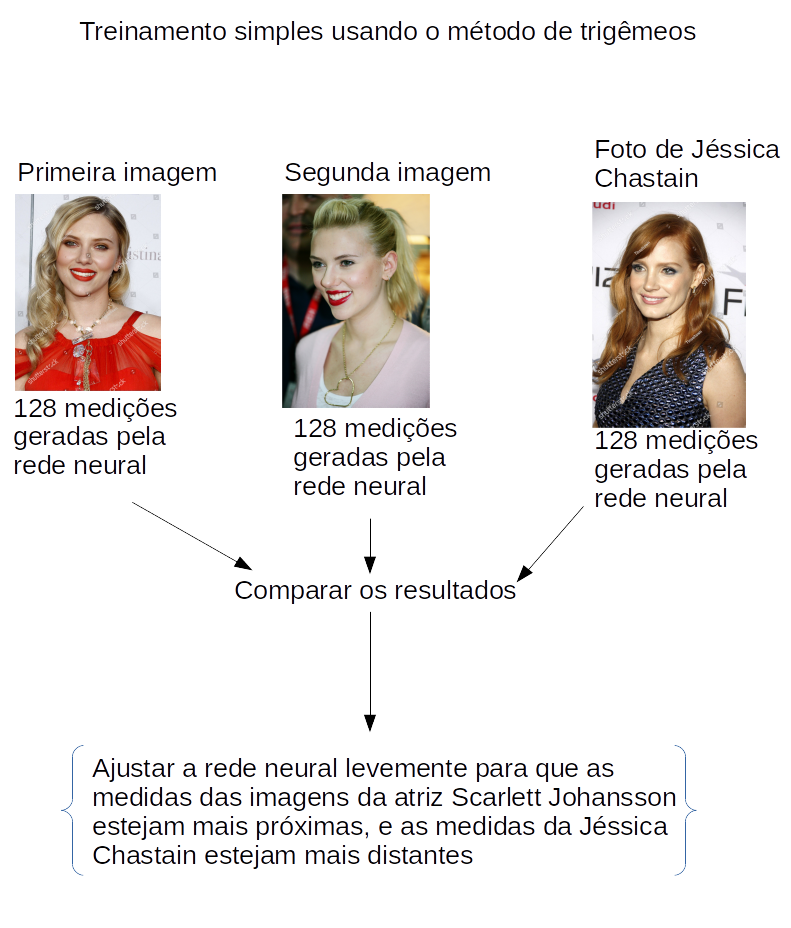
\includegraphics[scale=.4]{figs/atrizes.png}
  %\includesvg{figs/atrizes.svg}
  \legend{Fonte: o autor.}
  \label{fig:treinsimp}
\end{figure}
%-

Na ilustração \ref{fig:treinsimp} esta uma representação que mostra uma simulação muito simples de como funciona o método com trigêmeos, duas das trés faces são da atriz Scarlet Johansson que sera alvo no reconhecimento facial, e uma foto da atriz Jéssica Chastain que estará no nosso conjunto de dados. Então vamos considerar as faces, logo a ideia geral é que ajustaremos os pesos de nossa rede neural, para que as medias de 128-d das duas fotos da atriz Scarlet Johansson estejam o mais próximas o possível e mais distante da foto da Jéssica Chastain \cite{adamgeitgey}.

A técnica utilizada com a biblioteca (Dlib) e (Face Recognition) é baseada no (ResNet-34) do artigo “\textit{Deep Residual Learning for Image Recognition}” \cite{DBLP:journals/corr/HeZRS15}, mas com menos camadas e a metade do numero de filtros. 

A rede (Dlib) foi criada e treinada por Davis King em um conjunto de aproximadamente 3 milhões de imagens, ela pode chegar a um acerto comparado a outras técnicas de ponta de aproximadamente 99,38\% de precisão, e para concluir ela é uma rede (ResNet) com 29 camadas de convolução \cite{dlib1}.
%-
\begin{figure}[htpb]
  \centering
  \caption{Exemplo de comparação de vetores 128-d}
  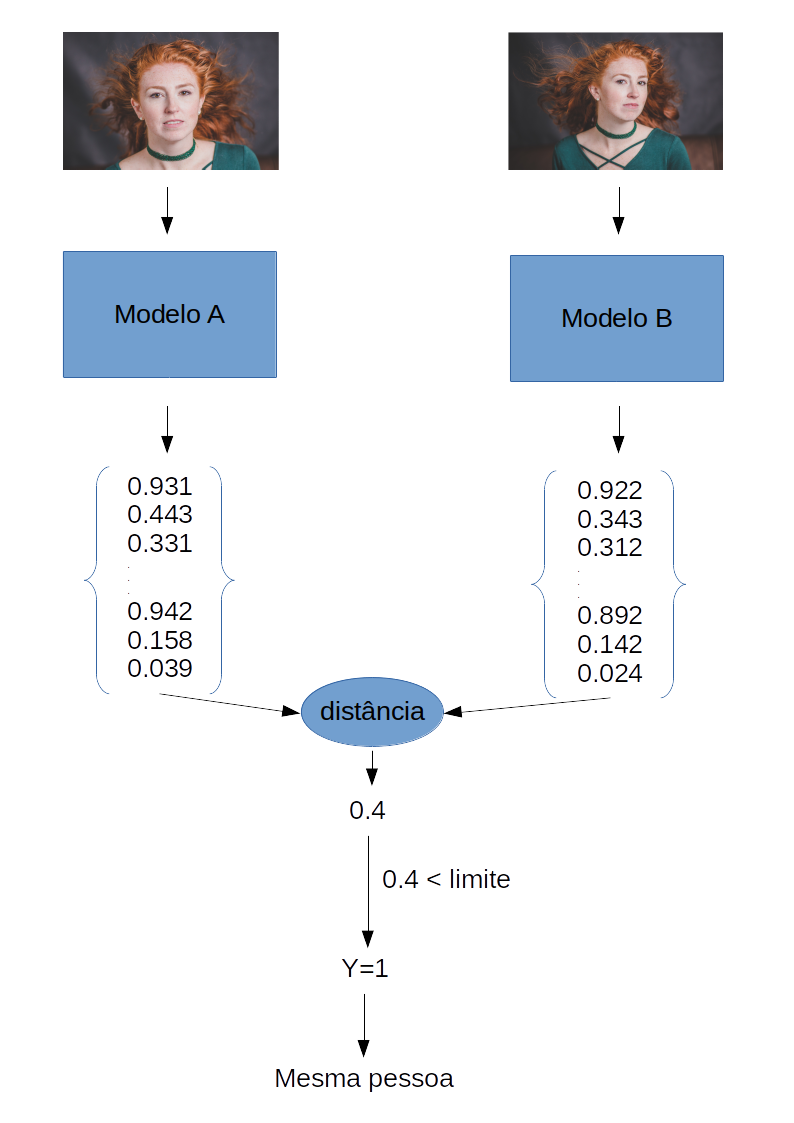
\includegraphics[scale=.5]{figs/gfdg.png}
  \legend{Fonte: o autor.}
  \label{fig:exetrein}
\end{figure}
%-

A figura \ref{fig:exetrein} é uma representação simples de como se chega a um resultado positivo no reconhecimento facial, como podemos ver os modelos pré-treinados já com seus respectivos pesos de vetores 128-d são comparados, e se perceber os seus valores numéricos são bem próximos, logo são comparados e como no exemplo da figura \ref{fig:exetrein} se seu resultado for inferior ao limite estipulado, isso indica que são imagens de uma mesma pessoa, gerando uma saída positiva ou variável Y=1 \cite{adamgeitgey}.

Na figura \ref{fig:ext128d} foi realizada uma simulação utilizando o método de codificação de uma face com reconhecimento facial para extração de um vetor 128-d, e ajustamos o algoritmo para mostrar em tela os pesos que foram encontrados. Ele gera exatamente 128 valores numéricos reais. 

%-
\begin{figure}[htpb]
  \centering
  \caption{Extração de um Vetor 128-d com Reconhecimento Facial}
  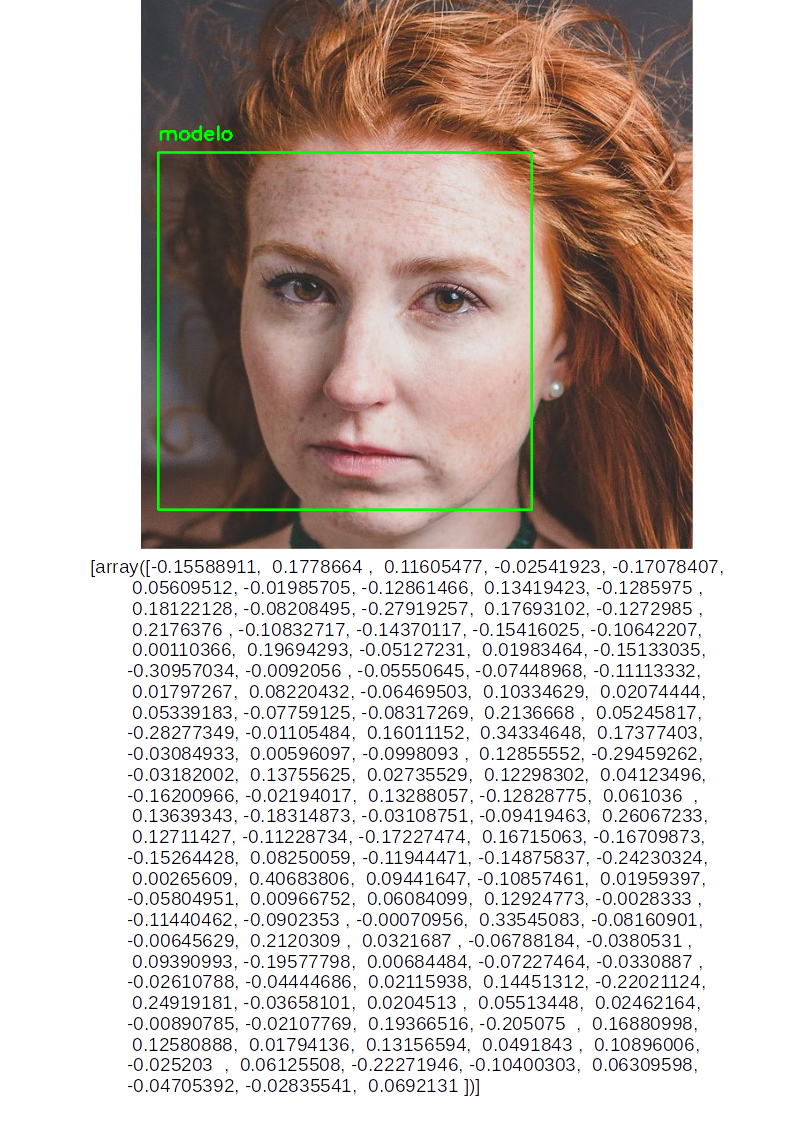
\includegraphics[scale=.5]{figs/modelo.png}
  \legend{Fonte: o autor.}
  \label{fig:ext128d}
\end{figure}

%-
\section{Tecnologias de Linguagem de Programação para Cálculos de Álgebra e Geometria}
%\addcontentsline{toc}{section}{Trabalhos Relacionados a Isto}

\subsection{Biblioteca NumPy}
%-
A biblioteca NumPy é hoje uma das principais ferramentas da linguagem Python utilizadas para cálculos numéricos e estruturas de dados, entre seus recursos ela possui cálculo de matrizes muito rápido e eficiente, funções que manipulam elementos da matriz e entre matrizes, possui ferramentas para leitura e gravação de dados de matrizes em disco, operações de álgebra linear, transformada de Fourier e uma confiável geração de números aleatórios [30]. 
Para o trabalho de movimentação do drone, ou seguir o objeto que será focado como o ator principal do trabalho é necessário saber a posição e coordenadas x e y dos pixels, isso é possível através de cálculos principalmente de matrizes, e para isso o OpenCV suporta a biblioteca NumPy.
 O NumPy é uma biblioteca altamente otimizada para operações numéricas, ele fornece uma sintaxe no estilo MATLAB. Todas as estruturas de matriz do OpenCV são convertidas para matrizes NumPy de e para ela. Portanto, quaisquer que sejam as operações que você possa realizar no NumPy, você pode combiná-lo com o OpenCV, o que aumenta o número de possibilidades. Além disso, várias outras bibliotecas como SciPy, que suporta NumPy podem ser usadas [15]. 

%-
\subsection{Biblioteca SciPy}
%-
A biblioteca SciPy juntamente com a NumPy se tornam uma ferramenta extremamente madura, avançada e confiável para processamento de aplicações cientificas. Há união dela com a NumPy estende muito além os recursos da NumPy, entre os recursos estão; Integração e derivações numéricas, decomposição de matrizes, solucionador de matrizes esparsas, e um grande conjunto de funções para trabalhar com cálculos que envolvem probabilidade e estatísticas. 
Na figura \ref{fig:desl} um breve exemplo de como serão utilizadas essas ferramentas de cálculo no protótipo [30].

\begin{figure}[htpb]
  \centering
  \caption{Exemplo de deslocamento utilizando calculos }
  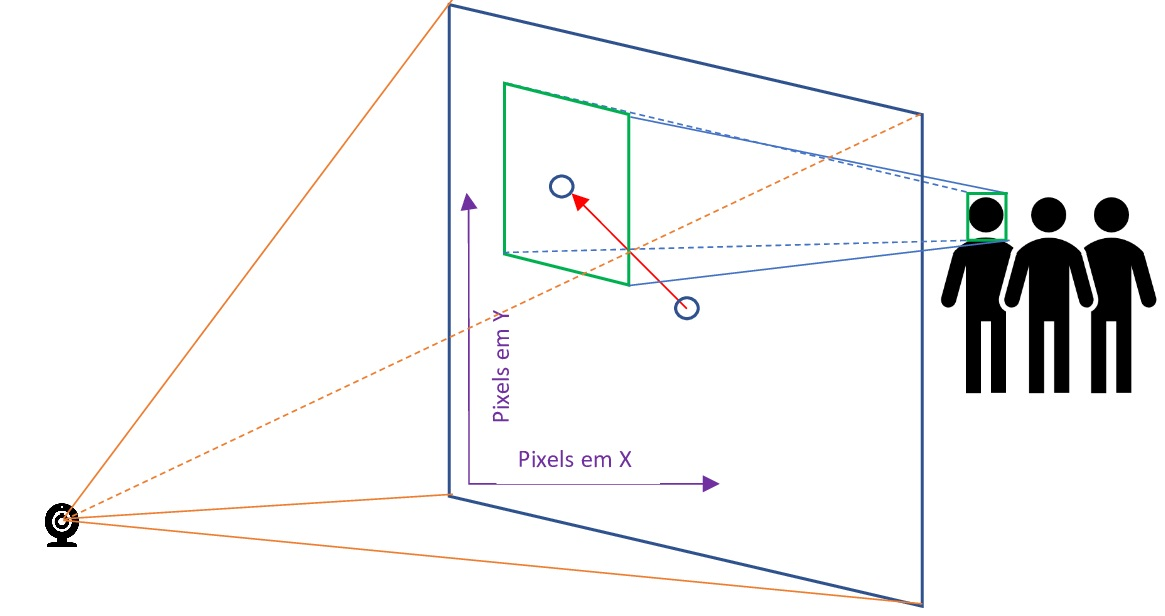
\includegraphics[scale=.5]{figs/rosto.jpg}
  \legend{Fonte: o autor.}
  \label{fig:desl}
\end{figure}
%-

A ideia é através das ferramentas de cálculo das bibliotecas conseguir os valores absolutos em pixels da imagem total captada pela câmera, e do retângulo que é desenhado em volta da face, e através de cálculos descobrir a direção o ângulo e o valor destes vetores direcionais (seta vermelha na figura) e aproximá-los através do deslocamento do drone.

\section{Tecnologias Open Source de Desenvolvimento, para Veículos Aéreos não Tripulados}

\subsection{Protocolo de Comunicação MAVLink}
%-
E possível criar uma ponte de comunicação entre o computador (Raspberry Pi) e a controladora de voo (Pixhawk), e com ele pode-se capturar pacotes da controladora de voo como por exemplo; registro de telemetria, altitude, velocidade do veículo.
Assim como se consegui capturar informações da controladora de voo, também é possível o contrário ou enviar comandos de voo do computador para a controladora. Todas essas informações trafegam através do protocolo de comunicação MAVLink.
O MAVLink é um protocolo de mensagens muito leve para comunicação em drones (e entre componentes de drones) [13].
O MAVLink segue um moderno padrão de design de publicação-assinatura e ponto a ponto híbrido: Os fluxos de dados são enviados/publicados como tópicos, enquanto os subprotocolo de configuração, como o protocolo de missão ou o parâmetro, são ponto a ponto com retransmissão [13].
As mensagens são definidas nos arquivos XML, cada arquivo XML define o conjunto de mensagens suportado por um sistema MAVLink específico, também conhecido como "dialeto". O conjunto de mensagens de referência implementado pela maioria das estações de controle de solo e pilotos automáticos é definido em common.xml (a maioria dos dialetos é construída sobre essa definição) [13].
A cadeia de ferramentas MAVLink usa as definições de mensagens XML para gerar bibliotecas MAVLink para cada uma das linguagens de programação suportadas. Drones, estações de controle de solo e outros sistemas MAVLink usam as bibliotecas geradas para se comunicar. Eles geralmente são licenciados pelo MIT e, portanto, podem ser usados sem limites em qualquer aplicativo de código fechado sem publicar o código-fonte do aplicativo de código fechado [13].

Características do MAVLink:
Muito eficiente; o MAVLink 1 possui apenas 8 bytes de sobrecarga por pacote, incluindo sinal de início e detecção de queda de pacote. O MAVLink 2 possui apenas 14 bytes de sobrecarga (mas é um protocolo muito mais seguro e extensível). Como o MAVLink não requer nenhum enquadramento adicional, é muito adequado para aplicativos com largura de banda de comunicação muito limitada.
Muito confiável;  MAVLink é usado desde 2009 para se comunicar entre vários veículos, estações terrestres (e outros nós) em canais de comunicação variados e desafiadores (alta latência / ruído). Ele fornece métodos para detectar quedas de pacotes, corrupção e autenticação de pacotes.
Suporta muitas linguagens de programação, executando em vários microcontroladores e sistemas operacionais (incluindo ARM7, ATMega, dsPic, STM32 e Windows, Linux, MacOS, Android e iOS).
Permite até 255 conexões simultâneas na rede (veículos, estações terrestres).
Permite comunicações externas e internas (por exemplo, entre um GCS e um drone, e entre o piloto automático do drone e a câmera do drone habilitada para MAVLink). A figura 6 demonstra o processo de comunicação juntamente com os processos de software, até gerar os dados de saída que são enviados para o drone por protocolo MAVLink.

%-
\subsection{Proxy de Protocolo MAVLink para Vant MAVProxy}
%-
O mavproxy e denominado de software para estação terrestre ou (GCS) ground station software, ele é totalmente funcional para o controle de (UAV) unmanned aerial vehicle ou veículo aéreo não tripulado, mas conhecido com drone. Ele foi desenvolvido pela CanberraUAV, é minimalista, portátil e extensível para qualquer UAV que suporte o protocolo MAVlink, visto no índice 1.3.1, um exemplo é o firmware ArduPilot que será abordado mais à frente. Ele foi desenvolvido para suportar computação complementar e vários datalinks, é hoje a ferramenta mais versátil para o controle e desenvolvimento de software baseados em drones, principalmente aqueles direcionados ao Ardupilot. Muitos recursos existentes em outras ferramentas GCS tem sua origem no MAVProxy [25]. O MAVProxy e liberado sobre a licença GNU (general public license) v3 ou superior.
Recursos:
\begin{itemize}
    \item É baseado em linha de comando muito focada em Linux. Existem plugins que fornecem uma GUI (graphical user interface).
    \item Poder ser executado em localhost ou em rede em vários computadores.
    \item Abrange as normas POSIX (portable operating system interface), ou roda em qualquer sistema operacional que tenha chamadas na linguagem python.
    \item Por ser muito leve roda muito bem em computadores com processamento limitado como o Raspberry Pi.
    \item Tab-completion of commands.
    \item Possui módulos carregáveis para várias tarefas como mapas, console, joysticks.
\end{itemize}
%-
\subsection{Ferramenta de Desenvolvimento para Vant Dronekit}
%-
O Dronekit é uma API feita para desenvolvedores criarem aplicativos que se comunicam com veículos (drone) por meio do MAVLink. É uma implementação em linguagem python para o controle de drones através de linguagem de programação, fornece acesso programático as informações de telemetria, estado e parâmetros a veículos conectados, permite o gerenciamento de missões e também o controle direto dos movimentos e operações do veículo.
O uso e direcionado diretamente a mini computadores como Raspberry Pi, Intel Edson, Nvidia TX1 para implementar funções adicionais que a controladora do drone não suporta, entre elas podemos citar a visão computacional e a modelagem 3D. Ele suporta Linux, Mac e Windows e é disponibilizado sobre a licença de código aberto Apache 2.0.

%-
\subsection{Simulador de Vant SITL}
%-
O simulador SITL (software in the loop) é uma ferramenta gráfica, no caso ele possui uma GUI (graphical user interface) que implementa a simulação de funcionamento total de um drone, ele permite utilizar um plane (avião), copter (drone) ou um rover (veículo terrestre), e isso sem a necessidade de nenhum hardware, resumindo ele permite testar o comportamento do código desenvolvido com o Dronekit em um simulador de drone assim evitando possíveis imprevistos que poderiam causar algum dano material ao seu equipamento real, seu drone físico. A figura \ref{fig:sitl} mostra um exemplo do simulador rodando em um ambiente Linux, ele demonstra um drone executando um script em python que se chama simple\_goto ou seja o script manda para o console do drone duas coordenadas para a qual ele deve viajar e logo em seguida retornar para a home (ponto de partida).

\begin{figure}[htpb]
  \centering
  \caption{Exemplo de Funcionamento do SITL}
  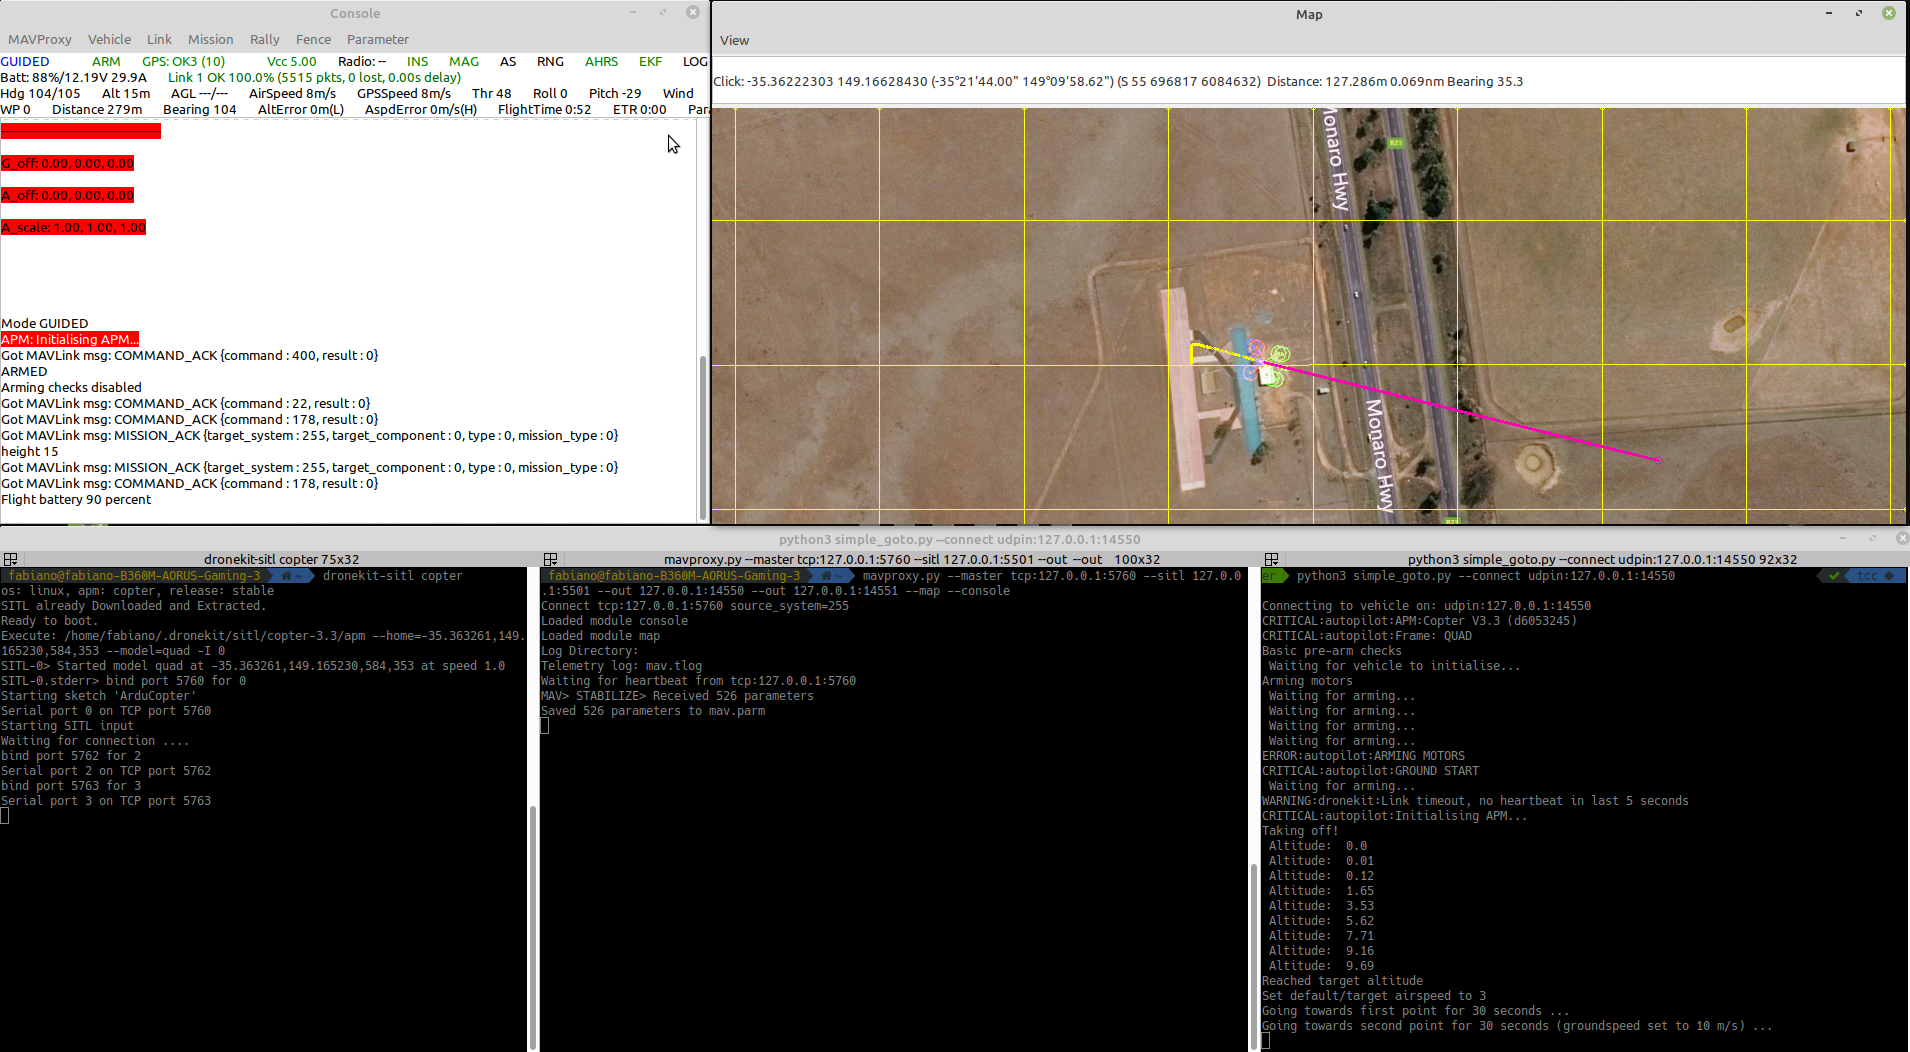
\includegraphics[scale=.3]{figs/sitl.png}
  \legend{Fonte: o autor.}
  \label{fig:sitl}
\end{figure}

O SITL permite executar o firmware Ardupilot diretamente no seu computador (nootbook, ou desktop), ele suporta várias plataformas entre elas Linux, Mac e Windows.
Com a junção do SITL e o Ardupilot se tem uma ampla gama de simuladores de veículos embutidos. Por exemplo:
\begin{itemize}
    \item Drone (multi-rotor)
    \item Aeronave de asa fixa
    \item Veículo terrestre
    \item Veículo subaquático
    \item Gimbal para suporte de câmera filmadora
    \item E uma ampla variedade de sensores como, Lidars e sensores óticos
\end{itemize}

Com eles se torna mais fácil o desenvolvimento de aplicativos para drone, isso porque dispõe de uma gama de ferramentas como, analisadores estáticos, depuradores interativos e análise dinâmica. A simulação é uma maneira rápida, fácil e segura de testar códigos implementados para o Ardupilot antes de tentar usar (voar) no mundo real. [26]. A figura \ref{fig:ardupilot} mostra o fluxo de funcionamento das intercomunicações entre os módulos para criar simulações de funcionamento de um drone.

\begin{figure}[htpb]
  \centering
  \caption{Fluxo de operação SITL, MAVProxy, Ardupilot e MAVLink}
  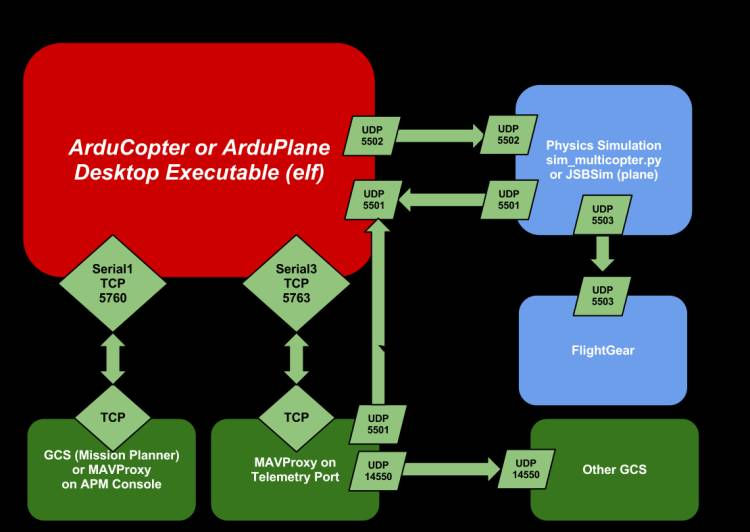
\includegraphics[scale=.5]{figs/ardupilot.jpg}
  \legend{Fonte: Ardupilot Documents, \cite{ardupilot}}
  \label{fig:ardupilot}
\end{figure}
%-
\subsection{Firmware para Vants}

\subsubsection{Ardupilot}
%-
Segundo a site do desenvolvedor, o Ardupilot é o software de piloto automático de código aberto mais avançado, completo e com mais recursos disponíveis. Foi desenvolvido ao longo de mais de 5 anos por uma equipe de diversos engenheiros profissionais e cientistas da computação. É o único software de piloto automático capaz de controlar qualquer sistema de veículo imaginável, de aviões convencionais, multirotores e helicópteros, barcos e até submarinos. E agora sendo expandido para oferecer suporte a novos tipos de veículos emergentes, como quadriciclos e helicópteros compostos [14].
Instalado em mais de um milhão de veículos em todo o mundo e com suas ferramentas avançadas de registro de dados, análise e simulação, o Ardupilot é o software de piloto automático mais testado e comprovado. A base de código-fonte aberto significa que está evoluindo rapidamente, sempre na vanguarda do desenvolvimento da tecnologia. Com muitos fornecedores periféricos criando interfaces, os usuários se beneficiam de um amplo ecossistema de sensores, computadores complementares e sistemas de comunicação. Por fim, como o código-fonte é aberto, ele pode ser auditado para garantir a conformidade com os requisitos de segurança e sigilo [14].
O pacote de software é instalado em aeronaves de muitas empresas como; 3DR, jDrones, PrecisionHawk, AgEagle e Kespry. Também é usado para testes e desenvolvimento por várias grandes instituições e corporações, como NASA, Intel, Boeing, além de inúmeras faculdades e universidades em todo o mundo [14].

%-
\subsection{Simulador de Robótica Gazebo}
%-
O Gazebo é um simulador de código aberto utilizado principalmente em robótica experimental, ele é um simulador muito bem projetado sendo assim tornando possível testar rapidamente algoritmos, projetar robôs, treinar sistema de IA usando cenários extremamente realísticos. O Gazebo possui um poderoso e robusto mecanismo de simulação física, ou seja, simula vários fenômenos físicos como; aceleração da gravidade, temperatura, pressão, luminosidade, e terrenos, também dispões de gráficos de alta qualidade e uma interface gráfica e programática [31]. 
%-
\subsection{Ferramenta para Desenvolvimento de Robótica ROS}
%-
O Ros é um sistema operacional de robótica de código aberto, com ele é possível desenvolver através de linguagem de programação, comportamentos de robôs para serem testados em um simulador como por exemplo o Gazebo. Uma das principais características do ROS e o reuso de código ele disponibiliza diversas aplicações prontas para o uso, essas aplicações simulam variados tipos de robôs, sensores, atuadores, câmeras e muito mais. Ele é implementado unicamente para o sistema operacional Linux, é baseado em versões e uma delas e a Melodic Morenia que é compatível com o Ubuntu Bionic [32].
%-
\section{Tecnologias e a Anatomia de Veículos Aéreos não Tripulados}
%-
Segundo a site do Ardupilot um drone ou multicoptero é um veículo aéreo mecanicamente simples, cujo movimento é controlado pela velocidade ou lentidão de várias unidades de motor/hélice para baixo.
Os multicoptero são aerodinamicamente instáveis e exigem absolutamente um computador de bordo (também conhecido como controlador de voo) para um voo estável. Como resultado, eles são sistemas "Fly by Wire" e se o computador não estiver funcionando, você não estará voando. O controlador de voo combina dados de pequenos giroscópios MEMs, acelerômetros (iguais aos encontrados em smartphones) para manter uma estimativa precisa de sua orientação e posição [14].

\begin{figure}[htpb]
  \centering
  \caption{Drone do Tipo Quadricóptero}
  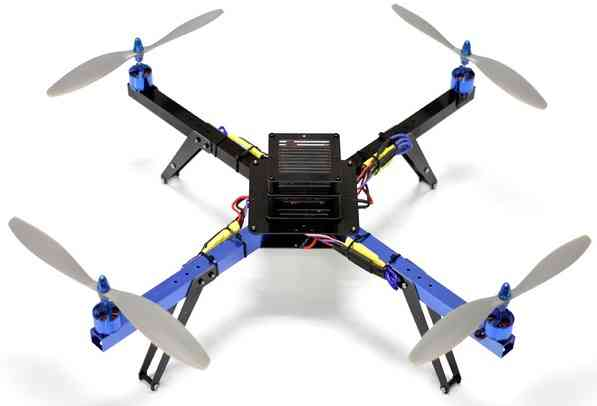
\includegraphics[scale=.5]{figs/drone.jpg}
  \legend{Fonte: Ardupilot Documents, \cite{ardupilot}}
  \label{fig:quad}
\end{figure}

O drone exemplo na figura \ref{fig:quad}, não será o foco do projeto porem será de importância impactante devido a sua necessidade para que o sistema projetado obtenha todas suas funcionabilidades. No caso do drone ele é o meio de transporte que dará aspecto de mobilidade para que seja possível se deslocar chegando ao foco do escopo, que no caso é seguir o objeto identificado pelo sistema de visão computacional.
Quando tudo estiver em funcionamento, fazendo com que o drone trabalhe de maneira autônoma ele deixara de ser um drone e se tornara um VANT (veículo aéreo não tripulado), e qual a diferença entre eles? Um drone se torna um VANT quando é capaz de vôo autônomo. Normalmente, isso significa pegar as informações de sensores como, acelerômetro e do giroscópio e combiná-las com os dados do barômetro e do GPS, para que o controlador de voo entenda não apenas sua orientação, mas também sua posição.

%-
\subsection{Frame}
%-
O frame é basicamente uma armação que pode ser de plástico, fibra de carbono, fibras entre outros materiais, possui alguns modelos como quadcoptero (quatro hélices), hexacoptero (seis hélices) octacoptero (oito hélices) [3]. A figura \ref{fig:frame} mostra um frame de um quadricóptero.

\begin{figure}[H]
  \centering
  \caption{Frame de um Vant Quadricóptero}
  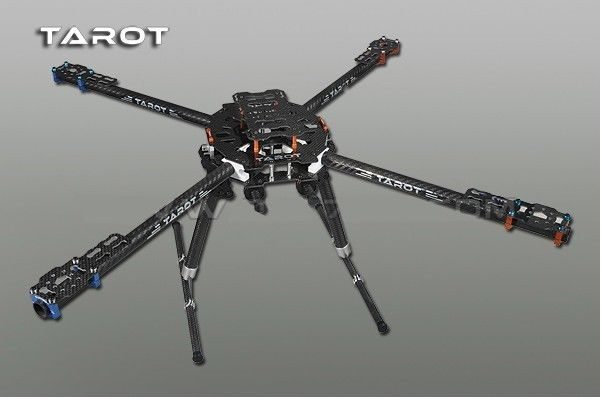
\includegraphics[scale=.5]{figs/frame.jpg}
  \legend{Fonte: Ardupilot Documents, \cite{ardupilot}}
  \label{fig:frame}
\end{figure}
%-
\subsection{Controladora de Voo}
%-
Uma controladora de voo é um hardware, é basicamente um equipamento físico composto por um circuito integrado o qual possui sensores como barômetro, gps, giroscópio, acelerômetros. Sensores que captam as atividades externas como a pressão do ar, posição geográfica, posição de equilíbrio em relação a gravidade (nivelamento), convertem essas atividades em sinais digitais e dessa forma a controladora juntamente com o firmware (Ardupilot/PX4) que possuem embarcado, conseguem interpretar esses sinais e utilizá-los para que consiga manter o equipamento em equilíbrio no ar, tornando ele um equipamento capaz de voar   e manter sua estabilidade [7].     
As controladoras de voo ou piloto automático são utilizadas para desenvolver equipamentos de controle remoto como drones, veículos terrestres, aviões e submersíveis aquáticos. Originalmente foram fabricadas e vendido pela 3DR, hoje é possível adquirir copias chinesas com custos bem mais em conta, devido ao projeto ser open source [3].
As figuras \ref{fig:pixhawk} e \ref{fig:pixhawkCirc} mostram a Pixhawk 1 uma das controladoras mais utilizadas.

\begin{figure}[htpb]
  \centering
  \caption{Pixhawk 1}
  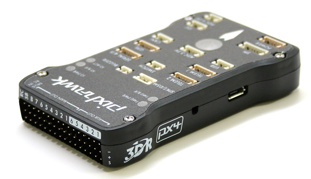
\includegraphics[scale=.7]{figs/pixhawk.png}
  \legend{Fonte: Ardupilot Documents, \cite{ardupilot}}
  \label{fig:pixhawk}
\end{figure}

\begin{figure}[htpb]
  \centering
  \caption{Diagrama eletrônico dos conectores da Pixhawk 1}
  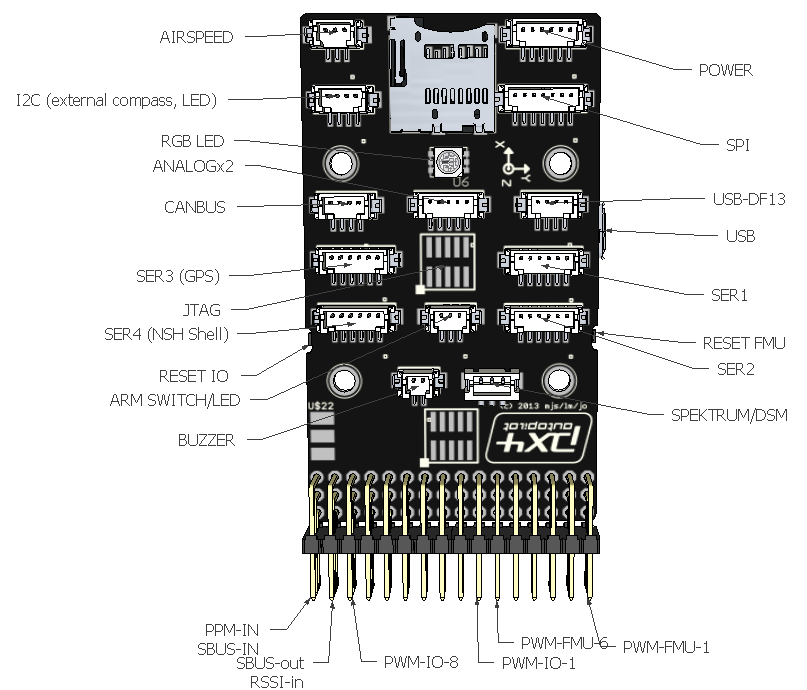
\includegraphics[scale=.4]{figs/Diagrama eletronico pixhawk.png}
  \legend{Fonte: Ardupilot Documents, \cite{ardupilot}}
  \label{fig:pixhawkCirc}
\end{figure}

\begin{itemize}

    \item Processador:
    \begin{itemize}
        \item Núcleo ARM Cortex M4 de 32 bits com FPU
        \item 168 Mhz / 256 KB de RAM / 2 MB Flash
        \item Co-processador à prova de falhas de 32 bits
        
    \end{itemize}
    
    \item Sensores:
    \begin{itemize}
        \item MPU6000 como principal acelerometro e giroscópio
        \item Giroscópio ST Micro de 16 bits
        \item Acelerômetro / bússola ST Micro de 14 bits (magnetômetro)
        \item Barômetro MEAS
    \end{itemize}
    
    \item Alimentação:
    \begin{itemize}
        \item Controlador de diodo ideal com failover automático
        \item Todas as saídas periféricas protegidas contra sobrecorrente, todas as entradas protegidas contra ESD
    \end{itemize}
    
    \item Interfaces:
    \begin{itemize}
        \item 5x portas seriais UART, 1 com capacidade de alta potência, 2 com controle de fluxo HW
        \item Entrada de Satélite Spektrum DSM / DSM2 / DSM-X
        \item Entrada Futaba S.BUS (saída ainda não implementada)
        \item Sinal de soma PPM
        \item Entrada RSSI (PWM ou tensão)
        \item I2C, SPI, 2x CAN, USB
        \item Entradas ADC de 3.3V e 6.6V
    \end{itemize}
    
    \item Dimensões:
    \begin{itemize}
        \item Peso 38g
        \item Largura 50 mm (2,0 pol.)
        \item Altura 15,5 mm (0,6 pol.)
        \item Comprimento 81,5 mm (3,2 pol.)
    \end{itemize}
     
\end{itemize}
%-
\subsection{Motor sem Escova}
%-
São motores de corrente elétrica continua de baixa tensão e sem escova, são síncronos e para funcionar nescessitam de um (drive) ou inversor de frequência [24]. A figura \ref{fig:motor} mostra um motor e na ilustração \ref{fig:motorpart} as partes internas.
\begin{figure}[H]
  \centering
  \caption{Motor sem Escova}
  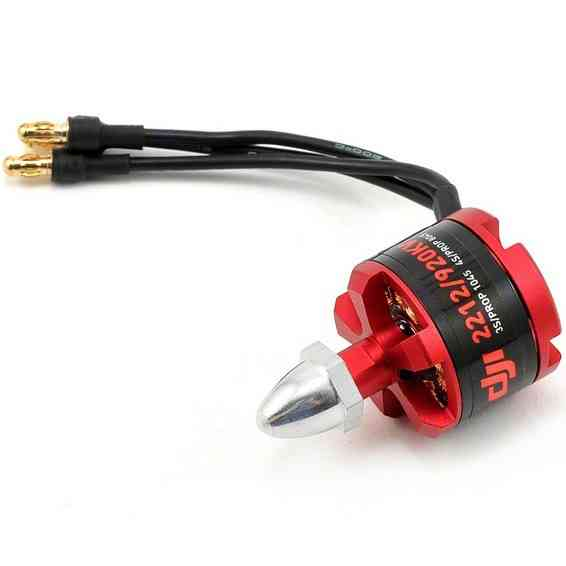
\includegraphics[scale=.3]{figs/brushless motor.jpg}
  \legend{Fonte: Ardupilot Documents, \cite{ardupilot}}
  \label{fig:motor}
\end{figure}

\begin{figure}[H]
  \centering
  \caption{Partes do Motor}
  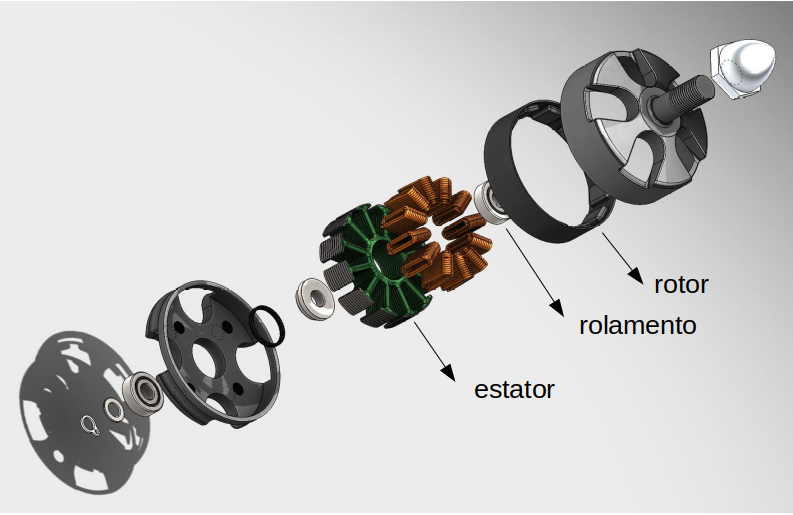
\includegraphics[scale=.4]{figs/motorexp.png}
  \legend{Fonte: o autor}
  \label{fig:motorpart}
\end{figure}
%-
%-
\subsection{Controlador Eletrônico de Correte (ESC)}
%-
Circuito eletrônico que controla a velocidade de rotação dos motores. A figura \ref{fig:esc} mostra um (ESC) muito utilizado em quadricópteros comuns e na ilustração \ref{fig:motordrive} o diagrama eletrônico.
\begin{figure}[H]
  \centering
  \caption{Controlador Eletrônico de Correte utilizado em Vants}
  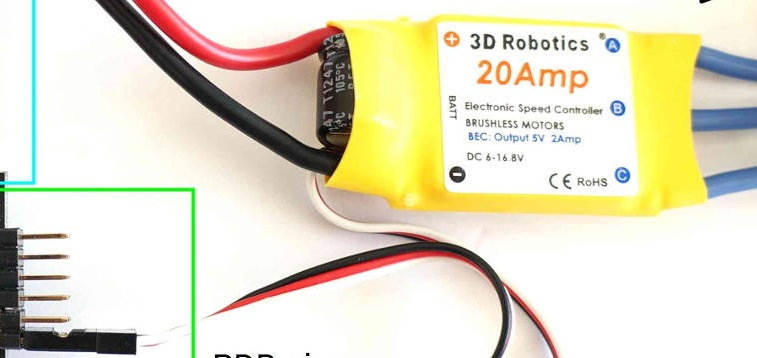
\includegraphics[scale=.3]{figs/esc.jpg}
  \legend{Fonte: Ardupilot Documents, \cite{ardupilot}}
  \label{fig:esc}
\end{figure}
%-

\begin{figure}[H]
  \centering
  \caption{Diagrama Eletrônico de um Controlador Eletrônico de Correte}
  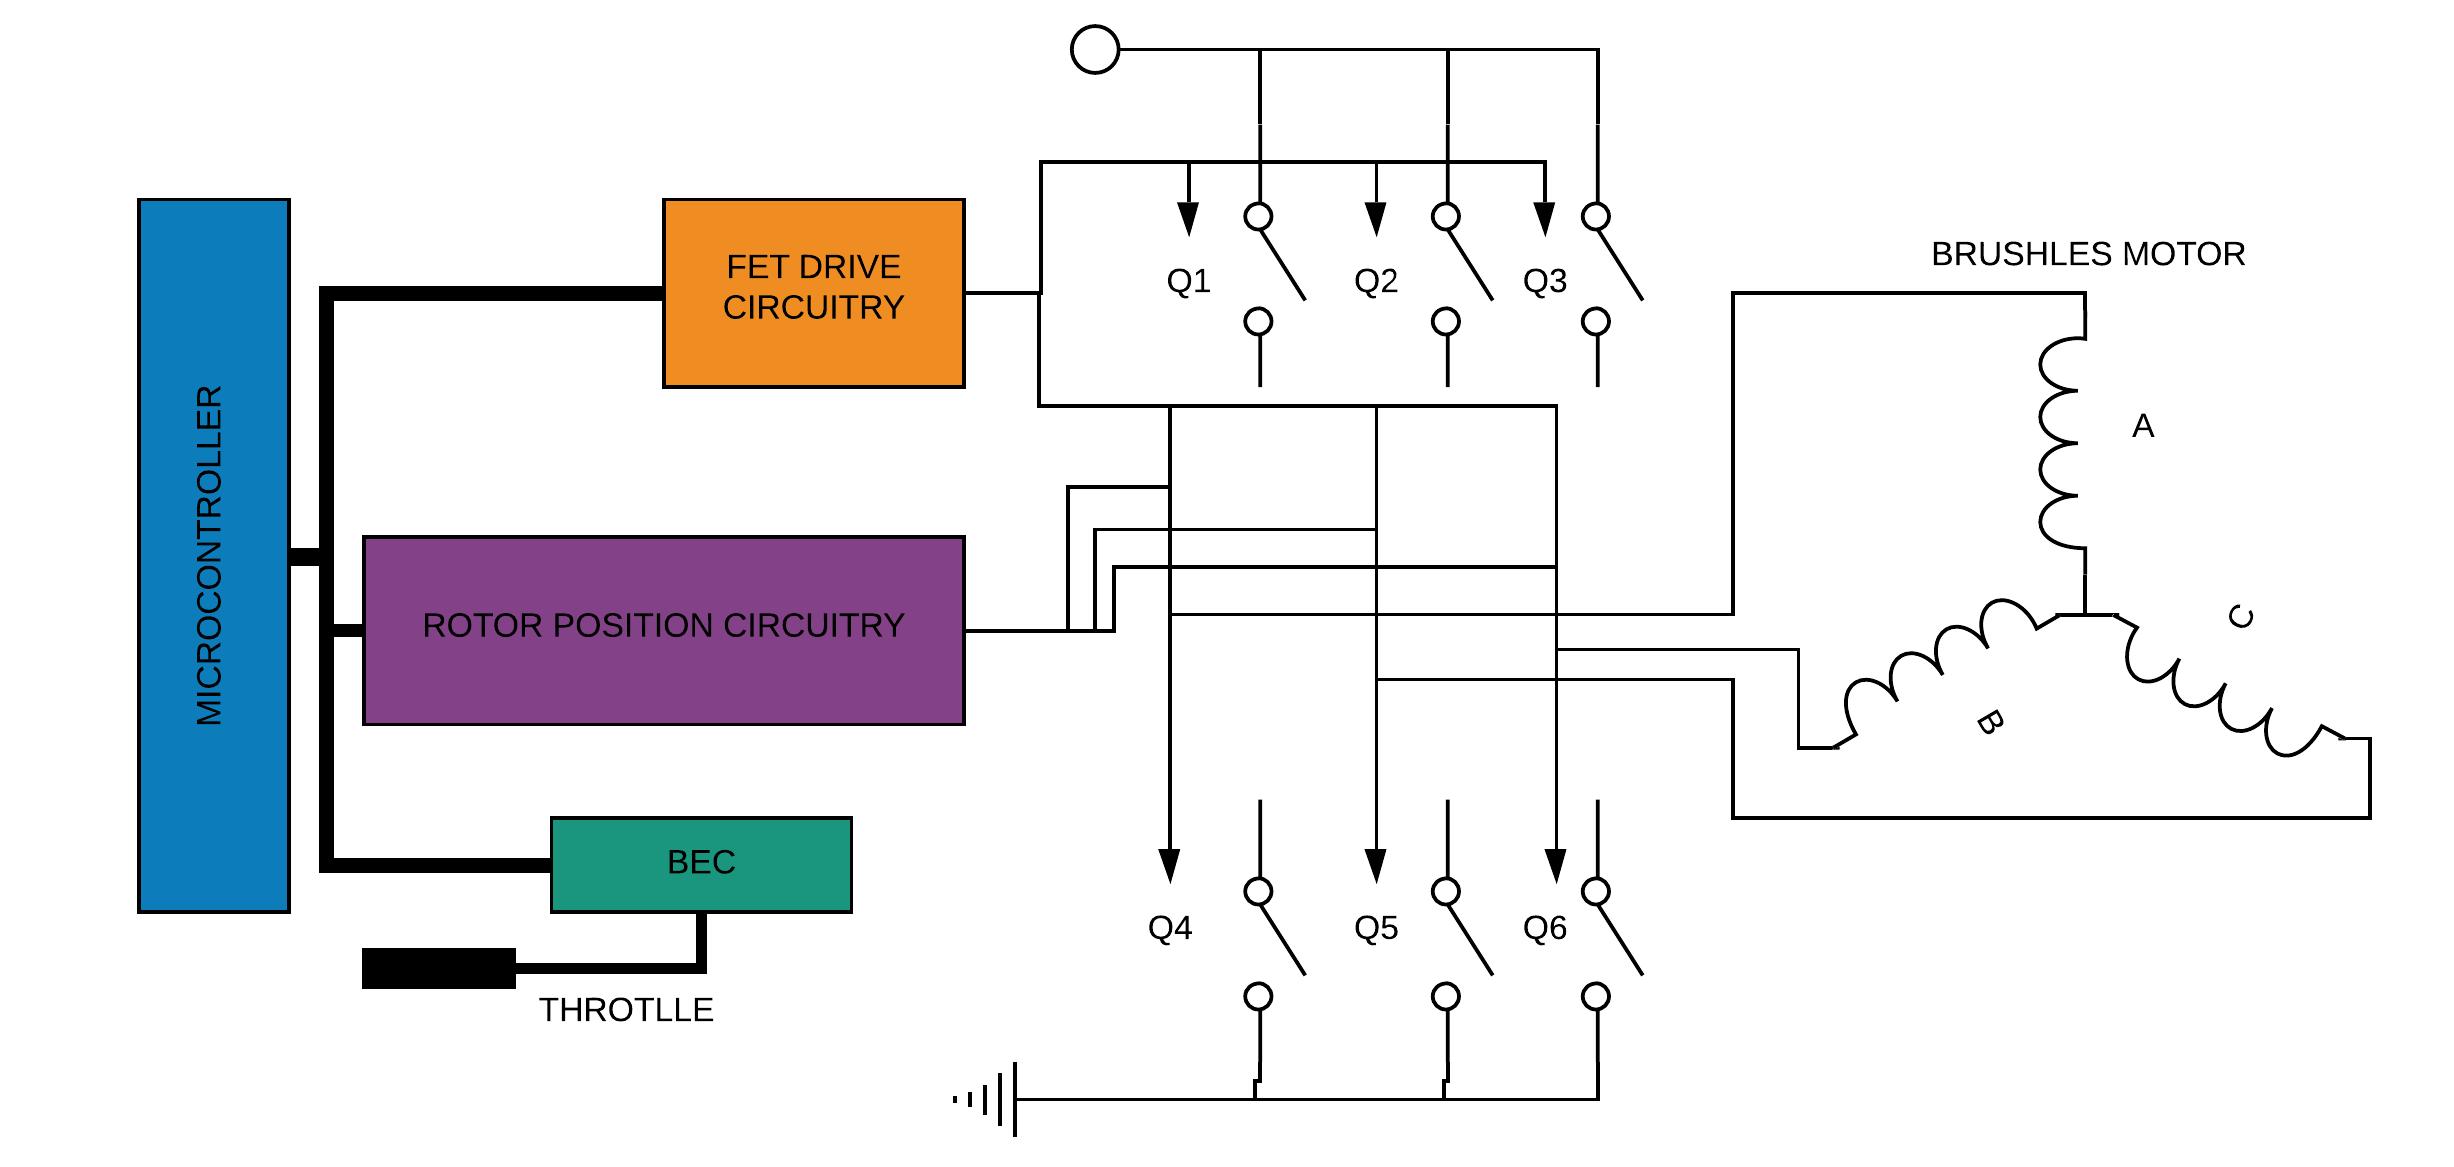
\includegraphics[scale=.2]{figs/drivemotorpng.png}
  \legend{Fonte: do autor, com base em \cite{motordrive}}
  \label{fig:motordrive}
\end{figure}
%-

\subsection{Módulo de GPS}
%-
Módulo de navegação GPS + Compass, é utilizado para a orientação do drone na superfície terrestre. A figura \ref{fig:gps} mostra um modulo de GPS.
\begin{figure}[H]
  \centering
  \caption{Modulo de GPS}
  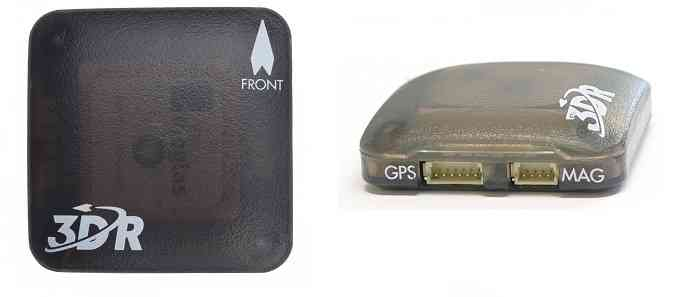
\includegraphics[scale=.8]{figs/gps.jpg}
  \legend{Fonte: Ardupilot Documents, \cite{ardupilot}}
  \label{fig:gps}
\end{figure}
%-
\subsection{Hélice}
%-
E um instrumento de propulsão ou tração, geralmente se acopla a um motor, ao girar empurra o que está na sua volta (ar ou água), assim converte energia rotacional em translacional, empurrando o objeto a que está engatada. Funcionam como asas e obedecem aos princípios de Bernoulli e a terceira lei de Newton. Podem ser fabricadas de resinas, plásticos, fibra de carbono entre outros materiais. A figura \ref{fig:helice} mostra um exemplo de uma hélice.
\begin{figure}[H]
  \centering
  \caption{Hélice}
  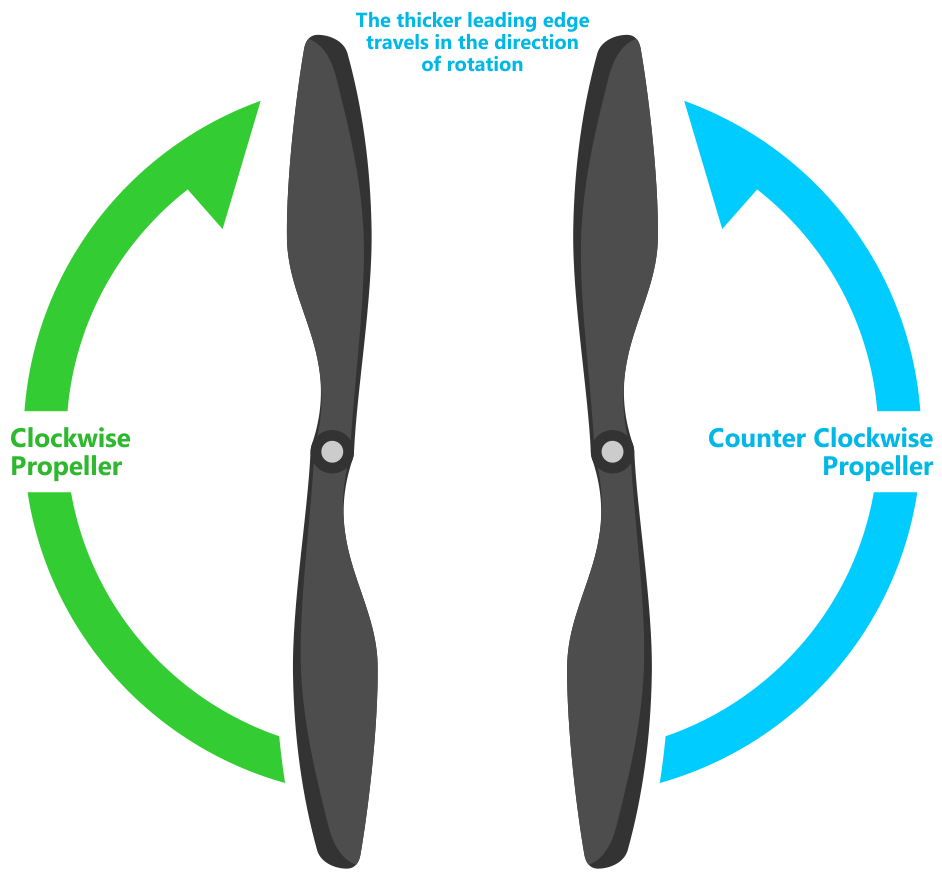
\includegraphics[scale=.7]{figs/helices.png}
  \legend{Fonte: Ardupilot Documents, \cite{ardupilot}}
  \label{fig:helice}
\end{figure}
%-
\subsection{Bateria de Polímero de Lítio (LíPo)}
%-
As baterias de polímero de lítio, são baterias que contêm sais de lítio num polímero solido como o oxido de polietileno em vez de solvente, isso as torna adaptáveis ou moldáveis a diferentes formatos. Cada célula tem tensão nominal de 3,7V, sendo que utilizam elas em série chegando a mais de uma especificação de alimentação, exemplo: 2s (duas células), 3s (três células). A figura \ref{fig:bat} mostra uma bateria do tipo LíPo 30c.
\begin{figure}[H]
  \centering
  \caption{Bateria de polímero de lítio}
  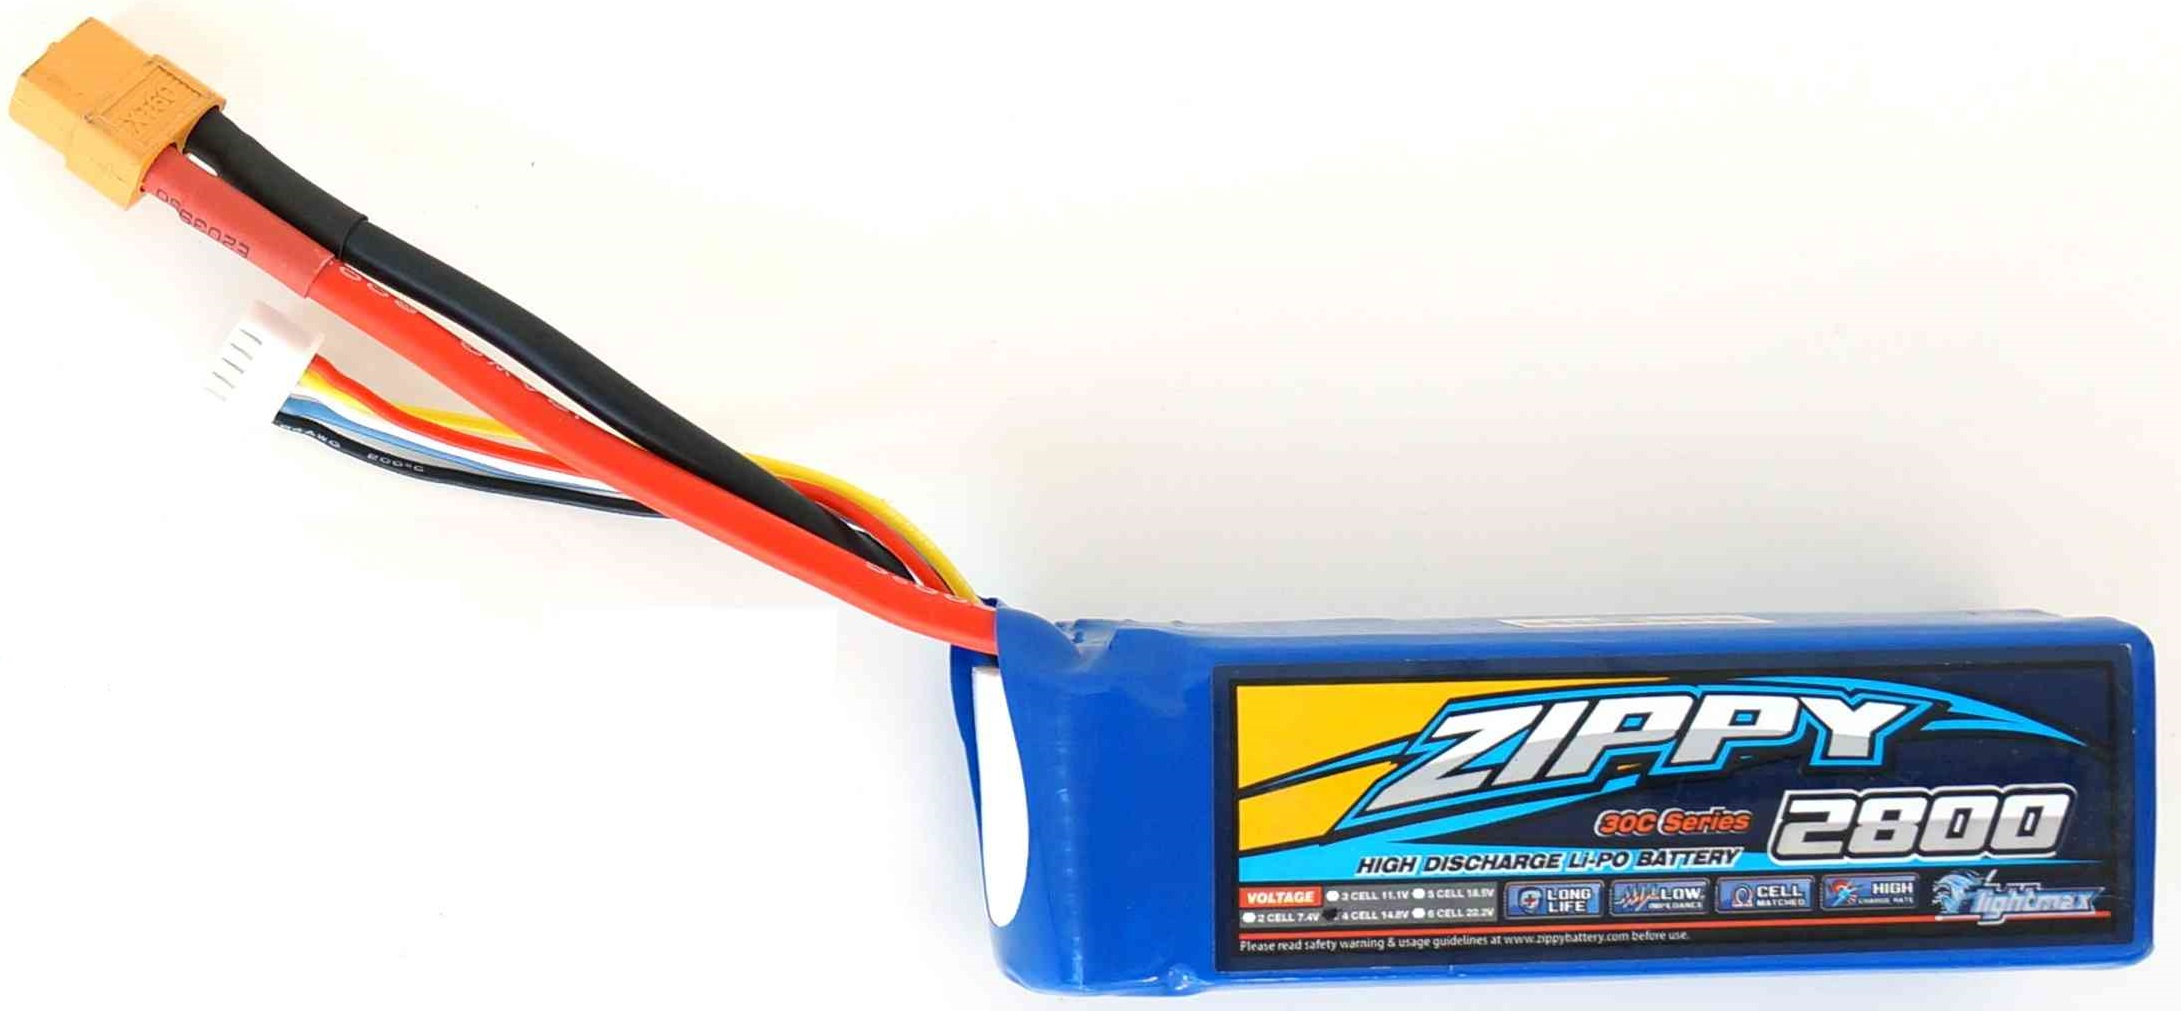
\includegraphics[scale=.2]{figs/bateria.jpg}
  \legend{Fonte: Ardupilot Documents, \cite{ardupilot}}
  \label{fig:bat}
\end{figure}
%-
\subsection{Esquema de Montagem de um Quadricóptero}
%-
\begin{figure}[H]
  \centering
  \caption{Esquema de Montagem de um drone}
  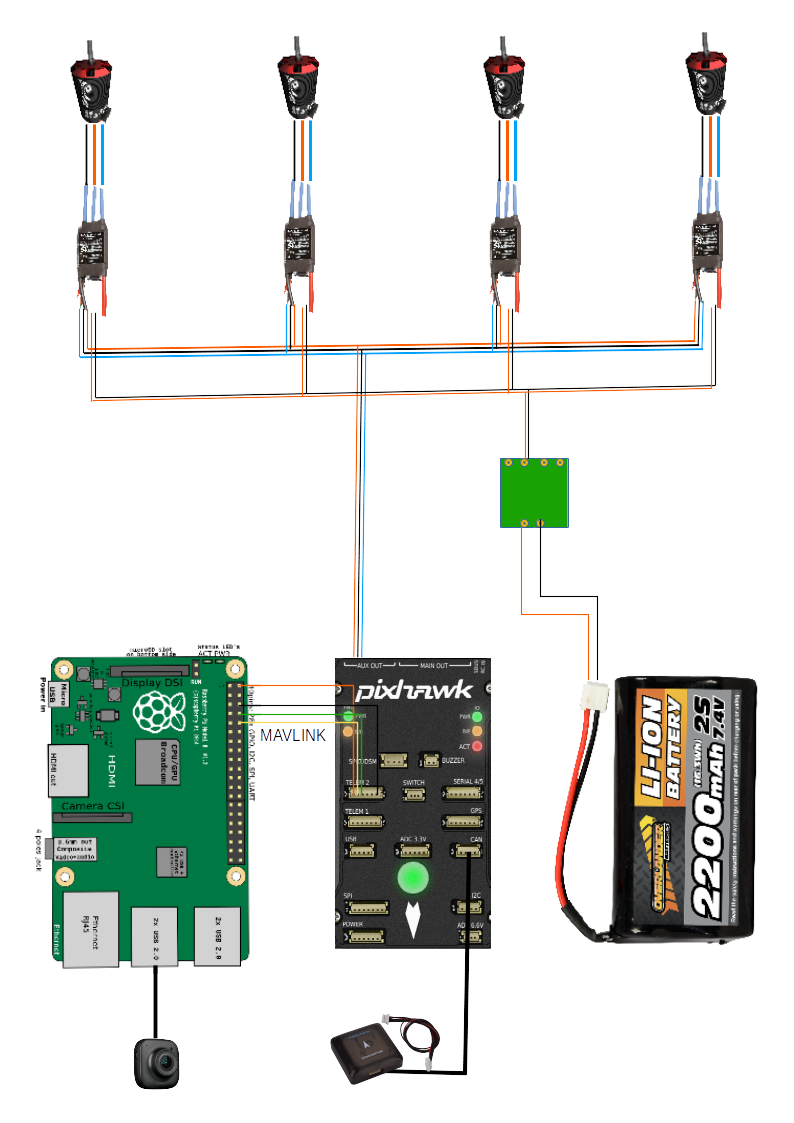
\includegraphics[scale=.5]{figs/esquema de ligacao do prototipo.png}
  \legend{Fonte: do autor}
  \label{fig:mount}
\end{figure}
%-
\section{Teoria de funcionamento e dinâmica de voo de um quadricóptero}

Para iniciar a explicação deste tópico poderíamos começar falando sobre alguma das leis de Newton ou demonstrar através de cálculos que toda a ação possui uma reação de mesma intensidade e diferente direções, porem a ideia é dar uma breve introdução das reações físicas que fazem com que um Vant do tipo quadricóptero voe. 

E para iniciar e preciso entender como uma estrutura do tipo hélice age para que consiga elevar e sustentar o Vant, e para isso será ilustrada a figura \ref{fig:asa} que mostra uma representação gráfica dessas reações. 

%-
\begin{figure}[htpb]
  \centering
  \caption{Teoria de sustentação de uma hélice}
  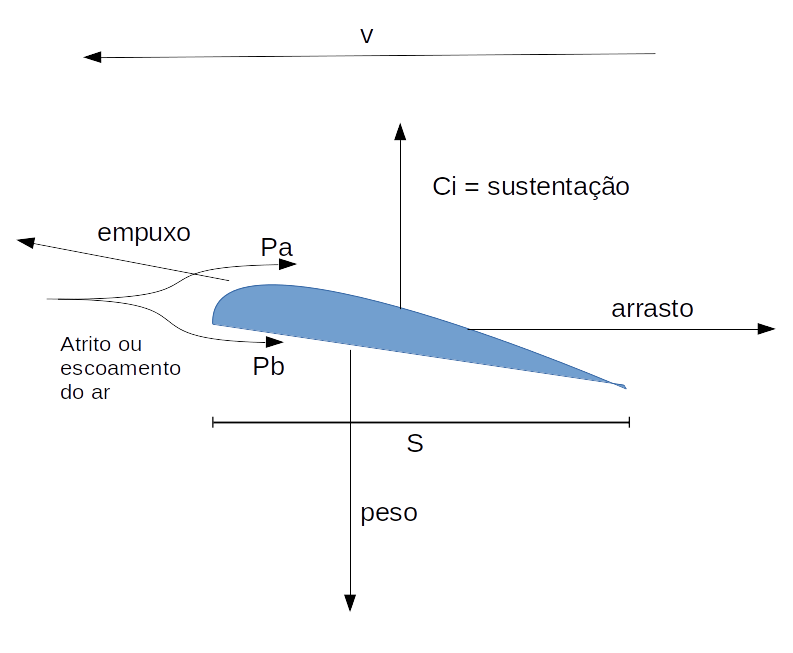
\includegraphics[scale=.4]{figs/helice.png}
  \legend{Fonte: do autor}
  \label{fig:asa}
\end{figure}
%-

Como pode se ver existem quatro reações principais, o empuxo, sustentação, peso e o arrasto, na figura \ref{fig:asa} Pb e Pa representam a pressão aplicada na hélice, na  parte de baixo da hélice Pb e na parte de cima Pa, essa pressão e exercida pelo deslocamento do ar que passa pela estrutura, basicamente a sustentação e acontece pela diferença de pressão entre Pa e Pb, e o design da estrutura que faz com que a velocidade do ar embaixo da estrutura seja maior do que em cima.

%-
\begin{itemize}
    \item Ci = coeficiente de sustentação;
    \item P = densidade do ar; 
    \item S = areá da superfície da asa;
    \item V = velocidade do ar; 
    \item L = força de sustentação;
\end{itemize}{}
%-
A equação \ref{sust} prova está sustentação: 

\begin{equation}
    \label{sust}
    L=Ci\left(\frac{p}{2}\right)Sv^2
\end{equation}

Existem outras equações matematísticas para calcular outras reações como o arrasto que seria a reação que puxa a estrutura na direção posterior da qual ela quer se deslocar ou então podemos dizer que é o rastro de ar que é deixado pela asa e tenta segura-lo, porem para este projeto é importante saber quais reações criam sustentação e fazem o veículo ganhar altitude vencendo a força da gravidade \cite{inproceedings}.
Agora vamos dar uma olhada nas reações que são aplicadas na estruturo do quadricóptero, como elas reagem juntamente com as reações de momento que a rotação do motor aplicam sobre a estrutura. E para expressar as reações a figura \ref{fig:esfcort} mostra elas graficamente. 

%-
\begin{figure}[htpb]
  \centering
  \caption{Diagrama de Esforços cortantes na Estrutura do Quadricóptero}
  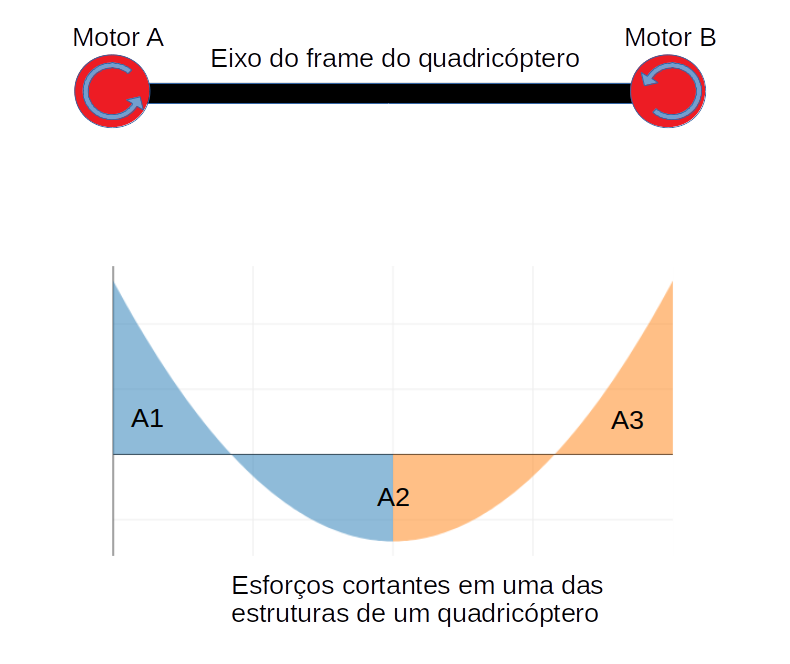
\includegraphics[scale=.3]{figs/esfcortante.png}
  \legend{Fonte: do autor}
  \label{fig:esfcort}
\end{figure}
%-

%-
\begin{figure}[htpb]
  \centering
  \caption{Diagrama de Momento Fletor sobre a Estrutura do Quadricóptero}
  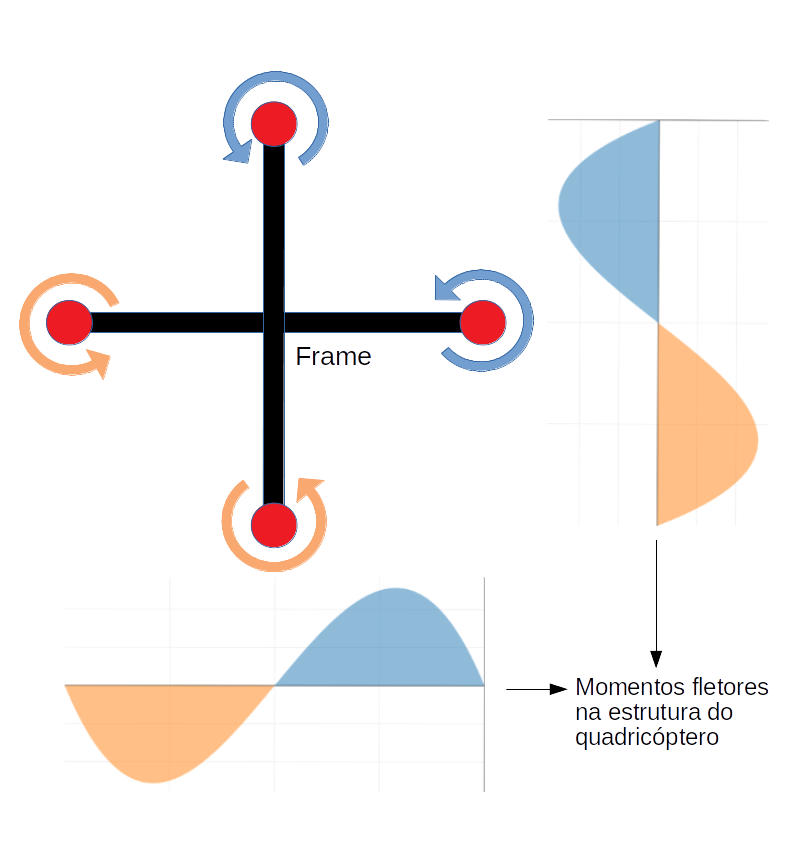
\includegraphics[scale=.3]{figs/momfletor.png}
  \legend{Fonte: do autor}
  \label{fig:momflet}
\end{figure}
%-

Na figura \ref{fig:esfcort} as reações que a rotação do motor geram na estrutura no frame dois pontos de esforço cortante, logo e possível observar que elas se cancelam, no caso a areá de  A1=A2 e A3=A2 o que faz com que elas se cancelem e com isso o equipamento não rotacione continuamente em um sentido. Já na figura \ref{fig:momflet} os gráficos de momento fletor demonstram que todas as forças no frame do quadricóptero acabam sempre se anulando. No ponto central do frame do quadricóptero o momento angular é zero dessa forma ele não rotaciona\cite{momesf}. 

%-
\begin{figure}[htpb]
  \centering
  \caption{Sentido de Movimento dos Motores e Inercias}
  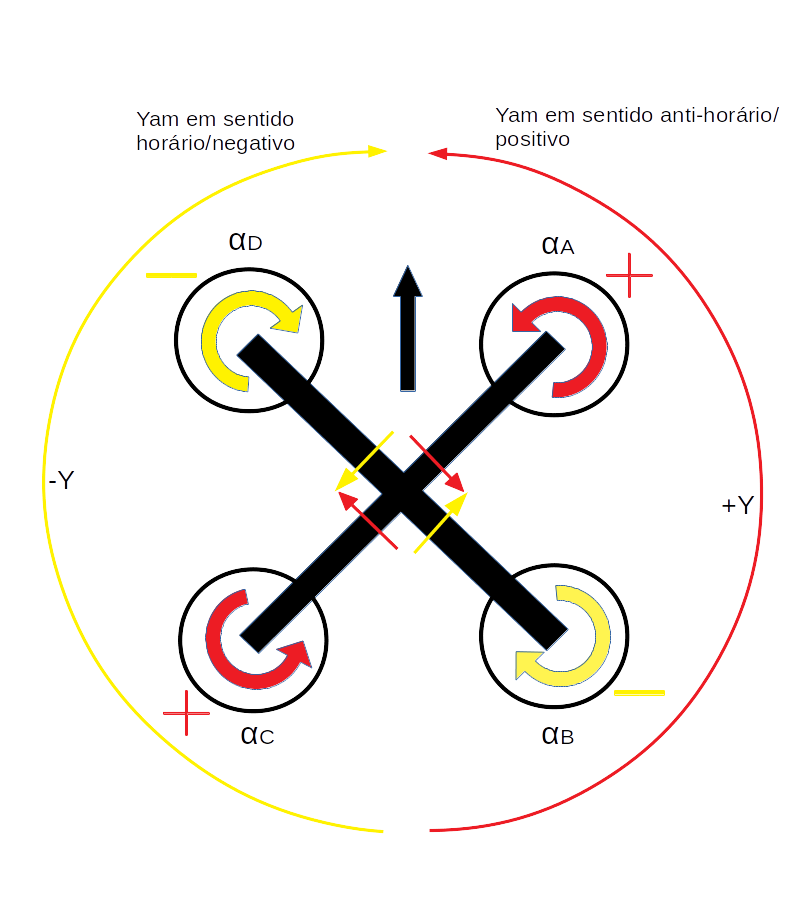
\includegraphics[scale=.3]{figs/rolldrone.png}
  \legend{Fonte: do autor}
  \label{fig:rotationmot}
\end{figure}
%-

No plano vertical um quadricóptero pode subir, descer e pairar, com isso é possível deduzir que para subir serão aplicadas forças nos motores de maneira que crie uma força ascendente que supere seu peso, e logo para pairar essas forças precisam se igualar ao máximo possível, mas tendo em mente que se igualarem é fisicamente impossível devido as varias reações da física que são exercidas no quadricóptero, logo para descer ele deve diminuir a velocidade de rotação dos motores de maneira que ascenda lentamente devido ao seu peso exercer empuxo gravitacional. 

Na pratica isso é simples os rotores giram jogando ar para baixo o ar empurra o equipamento para cima, e quem faz com que ele fique nivelado é a controladora de voo que simultaneamente com os sensores inerciais controlam a inclinação aplicando mais potência para cada motor independente de maneira que ele fique nivelado com a gravidade da terra, sim isso acontece muito rápido e freneticamente não é perceptível a olho nu \cite{forcecontrol}. 

Até aqui já sabemos como o quadricóptero sobe, desce,e paira, também sabemos o porque dele não girar em apenas um sentido, agora sera abordada a dinâmica do quadricóptero, ação que faz do quadricóptero um equipamento incrível, tendo capacidade de se movimentar rapidamente e em direções variadas, para quem não sabe é possível realizar uma manobra de "\textit{loop}" ou "\textit{flip}", é a capacidade de dar um giro muito rápido virando de ponta cabeça e voltando rapidamente a posição inicial. 

A figura \ref{fig:yamrollpitch} mostra todos os movimentos e seus respectivos nomes assim como são conhecidos, o "\textit{yam}" é o giro que o quadricóptero da em cima do seu próprio eixo pode ser em sentido horário e antiaéreo, "\textit{roll}" é uma inclinação lateral em relação a frente fazendo com que ele vá para a direita ou esquerda e logo o "\textit{pitch}" é a inclinação que faz com que ele se desloque na direção frontal ou traseira. 

%-
\begin{figure}[htb]
  \centering
  \caption{Movimentos de um Quadricóptero}
  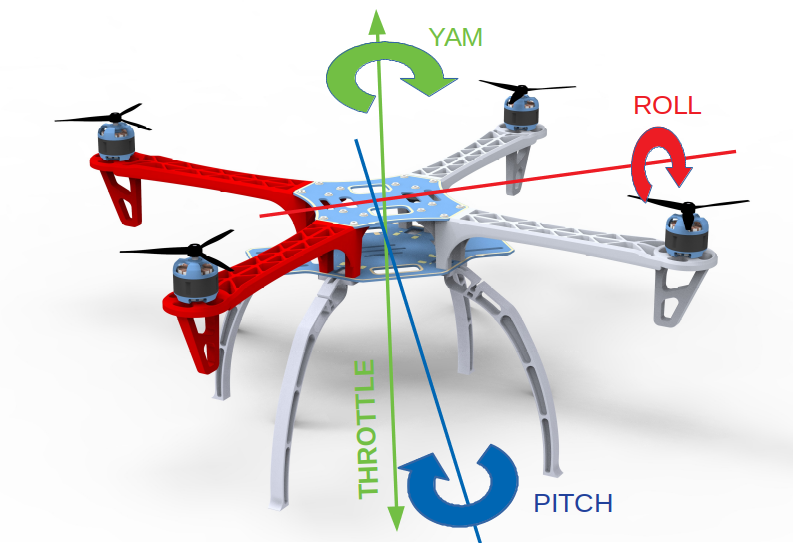
\includegraphics[scale=.3]{figs/F450.png}
  \legend{Fonte: do autor}
  \label{fig:yamrollpitch}
\end{figure}
%-

O Vant de quatro hélices possui basicamente dois movimentos que estimulam deslocamento, um deles é a guinada que faz com que ele se desloque horizontalmente dentro do plano cartesiano, já o movimento de giro ele rotaciona mudando a sua posição frontal e traseira respectivamente, muda o sentido de orientação da frente do equipamento como por exemplo de norte para leste e o sensor que rege esse movimento é a bussola do modulo de GPS. O movimento de giro acontece alterando a rotação dos motores, dois ao mesmo tempo no caso, um exemplo é como rotacionar ele no sentido horário. Perceba que na figura \ref{fig:rotationmot} $\alpha_{D}$ e $\alpha_{B}$ são negativos e $\alpha_{A}$ e $\alpha_{C}$ positivos, logo se atribuirmos a $\alpha_{D}$ e $\alpha_{A}$ um valor numérico 2 e a $\alpha_{C}$ e $\alpha_{B}$ o valor 2 igualmente chegaremos a um resultado zero o que indica que o Vant esta pairando sem girar.  

A soma dos torques dos motores gera a equação \ref{yam} que rege o movimento de Yam. 

\begin{equation}
    \label{yam}
    \left(k\right)\left(\alpha_{D}+\alpha_{A}-\alpha_{C}-\alpha_{B}\right)=Yd^2\left(\frac{\theta Y}{dt^2}\right)
\end{equation}

Vamos realizar outro exemplo de movimento, vamos supor que por exemplo queira girar para esquerda, segundo a figura \ref{fig:rotationmot} e a equação \ref{yam} atribuiremos para $\alpha_{C}$ e $\alpha_{A}$ o valor 3 e a $\alpha_{D}$ e $\alpha_{B}$ o valor 1, então chegaremos novamente a zero o que indica que o Vant esta estabilizado, porem a maior propulsão nos motores $\alpha_{B}$ e $\alpha_{D}$ faz com que ele gire no sentido anti-horário ou seu Y sera negativo como a ilustração \ref{fig:rotationmot} mostra \cite{momesf}.

A mesma equação apenas com uma pequena alteração pode ser aplicada para criar o movimento horizontal conhecido com "\textit{roll}". 

A soma dos momentos no centro de massa gera a equação \ que rege "\textit{roll}". 

\begin{equation}
    \label{roll}
    Lk\left(k\right)\left(\alpha_{D}+\alpha_{A}-\alpha_{C}-\alpha_{B}\right)=Rd^2\left(\frac{\theta R}{dt^2}\right)
\end{equation}

%-
\begin{figure}[htb]
  \centering
  \caption{Movimento horizontal "\textit{roll}"}
  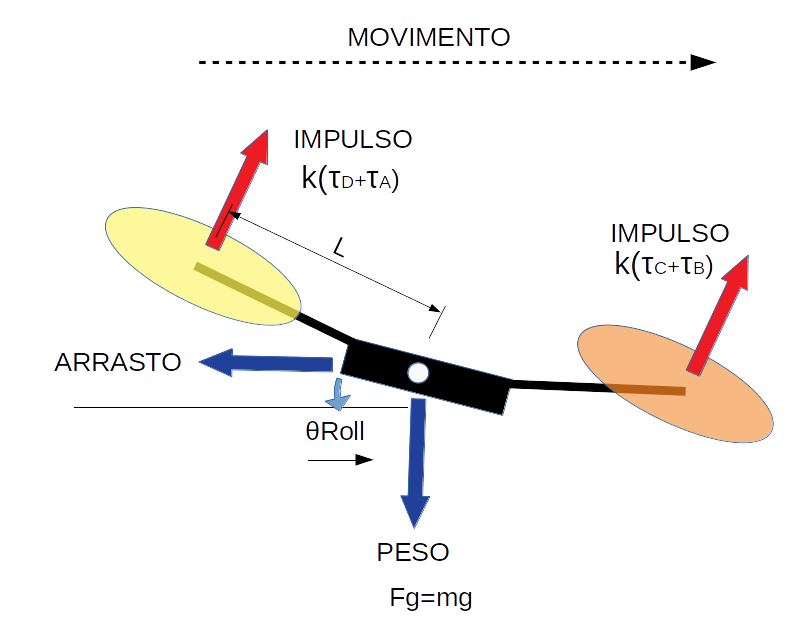
\includegraphics[scale=.3]{figs/dirdrone.png}
  \legend{Fonte: do autor}
  \label{fig:roll}
\end{figure}
%-

A figura \ref{fig:roll} ilustra uma vista lateral do movimento horizontal "\textit{roll}" e forças que o regem, perceba que o Vant esta inclinado mas como se consegue coloca-lo nesta posição? O aumento do impulso nos motores $\alpha_{C}$ e $\alpha_{B}$ e diminuição nos motores $\alpha_{D}$ e $\alpha_{A}$. O impulso total continua igual zero ou seu momento angular resulta em zero, porem a inclinação faz com que ele vá na direção em que esta inclinado, e a equação \ref{roll} e quem define esse movimento horizontal.
E para concluir a ilustração \ref{fig:dirdrone} denomina todos os movimentos horizontais de um quadricóptero \cite{calcmov}.  

%-
\begin{figure}[htb]
  \centering
  \caption{Movimentos horizontais de um quadricópter }
  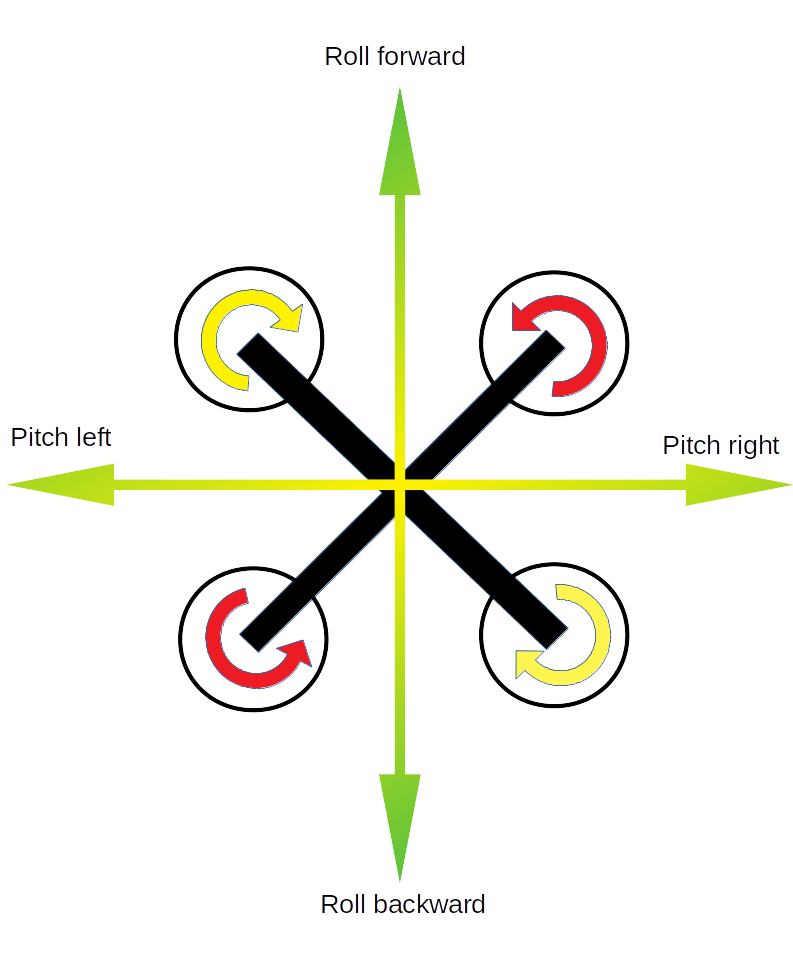
\includegraphics[scale=.3]{figs/sentido.png}
  \legend{Fonte: do autor}
  \label{fig:dirdrone}
\end{figure}
%-